\documentclass[a4paper,12pt]{article}
\usepackage[utf8]{inputenc}
\usepackage[pdftex]{graphicx}
\usepackage{wrapfig}
\usepackage{physics}
\usepackage{bbm}
\usepackage{pythonhighlight}
\usepackage{qcircuit}
\usepackage{lscape}
\usepackage[sort&compress,numbers]{natbib}
\usepackage{doi}
\bibliographystyle{apsrev4-1}
\newcommand{\bleq}{\ensuremath{\mathrel{\phantom{=}}}}
\newcommand{\nnl}{\nonumber\\}
\newcommand{\rme}{\mathrm{e}}
\newcommand{\rmi}{\mathrm{i}}
\newcommand{\R}{\mathbbm{R}}
\newcommand{\C}{\mathbbm{C}}
\newcommand{\Z}{\mathbbm{Z}}
\newcommand{\N}{\mathbbm{N}}
% Gates:
\newcommand{\hgt}{\mathrm{H}}
\newcommand{\igt}{\mathrm{I}}
\newcommand{\xgt}{\mathrm{X}}
\newcommand{\ygt}{\mathrm{Y}}
\newcommand{\zgt}{\mathrm{Z}}
\newcommand{\sgt}{\mathrm{S}}
\newcommand{\pgt}{\mathrm{P}}
\newcommand{\sdg}{\mathrm{S}^\dagger}
\newcommand{\sqx}{\sqrt{\mathrm{X}}}
\newcommand{\rz}{\mathrm{R_Z}}
\newcommand{\ry}{\mathrm{R_Y}}
%
\newcommand{\warning}[1]{{\bfseries\color{red}#1}}

\begin{document}
\title{Kagome VQE Notes}
\thispagestyle{empty}
\begin{center}
{\LARGE \bf Kagome VQE -- Notes}\\
\end{center}

\section{Hardware layout}

\subsection{Mapping Kagome to Guadalupe layout}

We can map the Kagome vertices and edges to the qubits of the Guadalupe device (cf. figure~\ref{fig:guadalupe}) as shown in figure~\ref{fig:kagome}.
\begin{figure}[h]
\centering
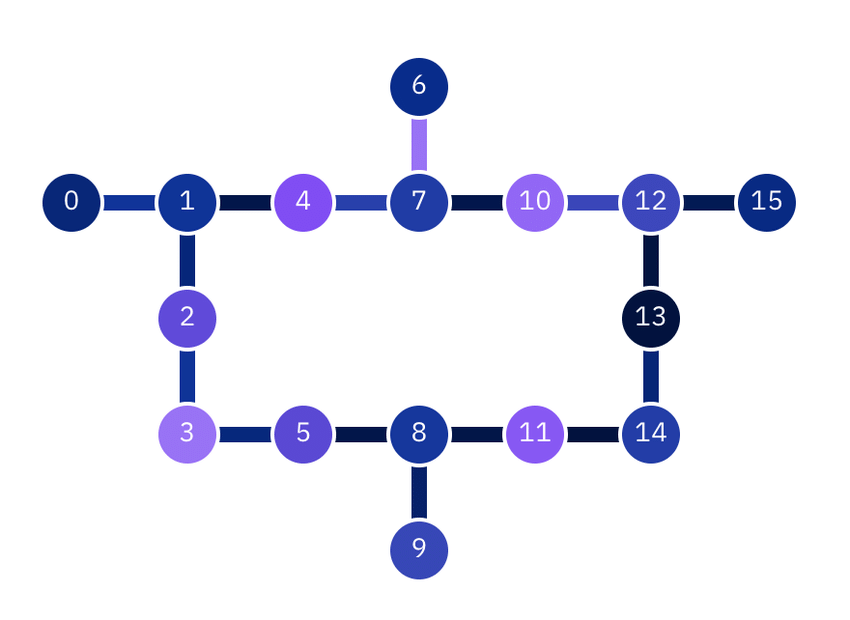
\includegraphics[width=80mm]{img/ibmq-guadalupe.png} 
\caption{Layout of the Guadalupe device\label{fig:guadalupe}}
\end{figure}

\begin{figure}[h]
\centering
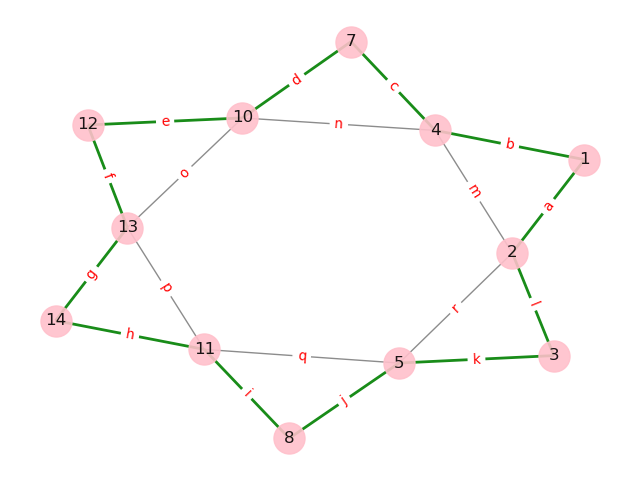
\includegraphics[width=120mm]{img/kagome.png}
\caption{Kagome unit cell. Numbers correspond to the qubits of the Guadalupe layout. Green edges correspond to physically connected qubits, whereas grey edges have no physical link and need to be achieved with swap gates.\label{fig:kagome}}
\end{figure}

\subsection{IBM hardware gates}
Note that IBM hardware implements $\rz$, $\sqx$, $\xgt$ and CNOT gates only. We can decompose:
\begin{equation}\begin{aligned}\label{eqn:hardware-gate}
 \hgt &= \rme^{\rmi \pi/4} \rz(\pi/2) \sqx \rz(\pi/2) \\
 \sgt &= \rme^{\rmi \pi/4}  \rz(\pi/2) \\
 \sdg &= \rme^{-\rmi \pi/4}  \rz(-\pi/2) \\
 \sgt\hgt &= \rme^{\rmi 3\pi/2}  \rz(-\pi) \sqx \rz(\pi/2) \\
 \hgt \sgt &= \rme^{\rmi 3\pi/2}  \rz(\pi/2) \sqx \rz(-\pi) \\
 \hgt \sdg &= \rz(\pi/2) \sqx \\
 \sdg \hgt &= \sqx \rz(\pi/2) 
\end{aligned}\end{equation}





\section{Unitaries}
Labeling edges with letters $a$..$r$ as shown in figure~\ref{fig:kagome}, we have the edge operators:
\begin{equation}\begin{aligned}
U_X^a(t) &= \exp(-\rmi t \xgt_1 \xgt_2) = \quad\begin{array}{c}
\Qcircuit @C=.5em @R=0.2em @!R {
\lstick{1} & \gate{\hgt} & \ctrl{1} & \qw & \ctrl{1} & \gate{\hgt} & \qw \\
\lstick{2} & \gate{\hgt} & \targ    & \gate{\rz(2t)} & \targ    & \gate{\hgt} & \qw
}
\end{array} \\
U_Y^a(t) &= \exp(-\rmi t \ygt_1 \ygt_2) = \quad\begin{array}{c}
\Qcircuit @C=.5em @R=0.2em @!R {
\lstick{1} & \gate{\sgt} & \gate{\hgt} & \ctrl{1} & \qw & \ctrl{1} & \gate{\hgt} & \gate{\sdg} & \qw \\
\lstick{2} & \gate{\sgt} & \gate{\hgt} & \targ    & \gate{\rz(2t)} & \targ    & \gate{\hgt} & \gate{\sdg} & \qw
}
\end{array} \\
U_Z^a(t) &= \exp(-\rmi t \zgt_1 \zgt_2) = \quad\begin{array}{c}
\Qcircuit @C=.5em @R=0.2em @!R {
\lstick{1} & \ctrl{1} & \qw & \ctrl{1} & \qw \\
\lstick{2} & \targ    & \gate{\rz(2t)} & \targ & \qw
}
\end{array}
\end{aligned}\end{equation}
and correspondingly $U_{X,Y,Z}^b(t)$ through $U_{X,Y,Z}^r(t)$ acting on the two qubit vertices given by the corresponding edge $b$..$r$.

Note that every single $U_\mu^\alpha(t)$ commutes with the total spins $S_x = \sum_{i=0}^{11} \xgt_i$, $S_y = \sum_{i=0}^{11} \ygt_i$, $S_z = \sum_{i=0}^{11} \zgt_i$, and therefore with $S^2 = S_x^2 + S_y^2 + S_z^2$.

We can combine these unitaries to a Heisenberg gate~\cite{kattemolleVariationalQuantumEigensolver2022}:
\begin{equation}\label{eqn:heisenberg}\begin{split}
U_H^a(\chi,\psi,\omega) = U_Z^a(\omega) U_Y^a(\psi) U_X^a(\chi)
\\= \quad\begin{array}{c}\tiny
\Qcircuit @C=.5em @R=0.2em @!R {
\lstick{1} & \gate{\mathrm{\rz}(\mathrm{\frac{\pi}{2}})} & \gate{\mathrm{\sqx}} & \gate{\mathrm{\rz}(\mathrm{\frac{\pi}{2}})} & \ctrl{1} & \qw & \ctrl{1} & \gate{\mathrm{\sqx}} & \ctrl{1} & \qw & \ctrl{1} & \gate{\mathrm{\rz}(\mathrm{\frac{\pi}{2}})} & \gate{\mathrm{\sqx}} & \ctrl{1} & \qw & \ctrl{1} & \qw & \qw\\
\lstick{2} & \gate{\mathrm{\rz}(\mathrm{\frac{\pi}{2}})} & \gate{\mathrm{\sqx}} & \gate{\mathrm{\rz}(\mathrm{\frac{\pi}{2}})} & \targ & \gate{\mathrm{\rz}(\mathrm{\chi})} & \targ & \gate{\mathrm{\sqx}} & \targ & \gate{\mathrm{\rz}(\mathrm{\psi})} & \targ & \gate{\mathrm{\rz}(\mathrm{\frac{\pi}{2}})} & \gate{\mathrm{\sqx}} & \targ & \gate{\mathrm{\rz}(\mathrm{\omega})} & \targ & \qw & \qw
}\end{array}\end{split}
\end{equation}


$U_{X,Y,Z}^a(t)$ through $U_{X,Y,Z}^l(t)$ can be directly implemented because the edges $a$..$l$ correspond to physical links. The operators on the edges $m$..$r$ must be implemented using SWAP gates:
\begin{equation}
 U_X^m(t) = \quad\begin{array}{c}
\Qcircuit @C=.5em @R=0.2em @!R {
\lstick{4} & \qw & \qw  & \qw  & \qw & \multigate{1}{U_X(t)} & \qw & \qw  & \qw  & \qw \\
\lstick{1} & \ctrl{1} & \targ    & \ctrl{1} & \qw & \ghost{U_X(t)} & \ctrl{1} & \targ    & \ctrl{1} & \qw \\
\lstick{2} & \targ    & \ctrl{-1} & \targ   &  \qw  &  \qw & \targ    & \ctrl{-1} & \targ   &  \qw
}\end{array}
\end{equation}
and correspondingly for all $U_{X,Y,Z}^m(t)$ through $U_{X,Y,Z}^r(t)$.

We can group these 54 operators into:
\begin{equation}\label{eqn:ux1groups}\begin{aligned}
U_X^1 &= U_X^a(\chi_a) U_X^c(\chi_c) U_X^e(\chi_e) U_X^g(\chi_g) U_X^i(\chi_i) U_X^k(\chi_k) \\
U_Y^1 &= U_Y^a(\psi_a) U_Y^c(\psi_c) U_Y^e(\psi_e) U_Y^g(\psi_g) U_Y^i(\psi_i) U_Y^k(\psi_k) \\
U_Z^1 &= U_Z^a(\omega_a) U_Z^c(\omega_c) U_Z^e(\omega_e) U_Z^g(\omega_g) U_Z^i(\omega_i) U_Z^k(\omega_k) \\
%
U_X^2 &= U_X^b(\chi_b) U_X^d(\chi_d) U_X^f(\chi_f) U_X^h(\chi_h) U_X^j(\chi_j) U_X^l(\chi_l) \\
U_Y^2 &= U_Y^b(\psi_b) U_Y^d(\psi_d) U_Y^f(\psi_f) U_Y^h(\psi_h) U_Y^j(\psi_j) U_Y^l(\psi_l) \\
U_Z^2 &= U_Z^b(\omega_b) U_Z^d(\omega_d) U_Z^f(\omega_f) U_Z^h(\omega_h) U_Z^j(\omega_j) U_Z^l(\omega_l) \\
%
U_X^3 &= U_X^m(\chi_m) U_X^o(\chi_o) U_X^q(\chi_q) \\
U_Y^3 &= U_Y^m(\psi_m) U_Y^o(\psi_o) U_Y^q(\psi_q) \\
U_Z^3 &= U_Z^m(\omega_m) U_Z^o(\omega_o) U_Z^q(\omega_q) \\
%
U_X^4 &= U_X^n(\chi_n) U_X^p(\chi_p) U_X^r(\chi_r) \\
U_Y^4 &= U_Y^n(\psi_n) U_Y^p(\psi_p) U_Y^r(\psi_r) \\
U_Z^4 &= U_Z^n(\omega_n) U_Z^p(\omega_p) U_Z^r(\omega_r) 
\end{aligned}\end{equation}
where each $U^i_{X,Y,Z}$ contains only mutually commuting terms.

We can group these further to
\begin{equation}\begin{aligned}
U_X(\vec\chi) &= U_X^1 U_X^2 U_X^3 U_X^4 \\
U_Y(\vec\psi) &= U_Y^1 U_Y^2 U_Y^3 U_Y^4 \\
U_Z(\vec\omega) &= U_Z^1 U_Z^2 U_Z^3 U_Z^4
\end{aligned}\end{equation}
each of which contains mutually commuting terms. $\vec\chi$, $\vec\psi$, and $\vec\omega$ denote vectors of the $3 \times 18$ parameters $\chi_{a..r}$, $\psi_{a..r}$, and $\omega_{a..r}$, respectively. With the representation in the hardware native gates~\eqref{eqn:hardware-gate}, these circuits have depths
\begin{equation}\begin{aligned}
\text{depth}(U_X) &= 4 \times 9 + 12 = 48 \\
\text{depth}(U_Y) &= 4 \times 8 + 12 = 44 \\
\text{depth}(U_Z) &= 4 \times 3 + 12 = 24 \,,
\end{aligned}\end{equation}
amounting to a total depth of 116 per layer.

Using, instead, the Heisenberg gate~\eqref{eqn:heisenberg} for a grouping into four groups $U_H^i = U_Z^i U_Y^i U_X^i$ as given in equation~\eqref{eqn:ux1groups} results in flatter circuits
\begin{equation}
U_H^1(\vec\theta_1) = \qquad \begin{array}{c}
\Qcircuit @C=.5em @R=0.2em @!R {
\lstick{2} & \multigate{1}{U_H(\chi_a,\psi_a,\omega_a)} & \qw \\
\lstick{1} & \ghost{U_H(\chi_a,\psi_a,\omega_a)} & \qw \\
\lstick{4} & \multigate{1}{U_H(\chi_c,\psi_c,\omega_c)} & \qw \\
\lstick{7} & \ghost{U_H(\chi_c,\psi_c,\omega_c)} & \qw \\
\lstick{10} & \multigate{1}{U_H(\chi_e,\psi_e,\omega_e)} & \qw \\
\lstick{12} & \ghost{U_H(\chi_e,\psi_e,\omega_e)} & \qw \\
\lstick{13} & \multigate{1}{U_H(\chi_g,\psi_g,\omega_g)} & \qw \\
\lstick{14} & \ghost{U_H(\chi_g,\psi_g,\omega_g)} & \qw \\
\lstick{11} & \multigate{1}{U_H(\chi_i,\psi_i,\omega_i)} & \qw \\
\lstick{8} & \ghost{U_H(\chi_i,\psi_i,\omega_i)} & \qw \\
\lstick{5} & \multigate{1}{U_H(\chi_k,\psi_k,\omega_k)} & \qw \\
\lstick{3} & \ghost{U_H(\chi_k,\psi_k,\omega_k)} & \qw 
}\end{array} \,,
\end{equation}
where $\vec\theta_1$ is a vector of the 18 parameters entering in the definition of $U_H^1$,
and correspondingly for $U_H^2(\vec\theta_2)$ with all 2-qubit gates shifted by one position. The inner edges result in
\begin{equation}
U_H^3(\vec\theta_3) = \qquad \begin{array}{c}
\Qcircuit @C=.5em @R=0.2em @!R {
\lstick{2} & \ctrl{1} & \targ     & \ctrl{1} & \qw & \ctrl{1} & \targ     & \ctrl{1} & \qw \\
\lstick{1} & \targ    & \ctrl{-1} & \targ &\multigate{1}{U_H(\chi_m,\psi_m,\omega_m)} & \targ    & \ctrl{-1} & \targ & \qw \\
\lstick{4} & \qw & \qw & \qw & \ghost{U_H(\chi_m,\psi_m,\omega_m)} & \qw & \qw & \qw & \qw \\
%
\lstick{7} & \qw & \qw & \qw & \qw & \qw & \qw & \qw & \qw \\
%
\lstick{10} & \ctrl{1} & \targ     & \ctrl{1} & \qw & \ctrl{1} & \targ     & \ctrl{1} & \qw \\
\lstick{12} & \targ    & \ctrl{-1} & \targ &\multigate{1}{U_H(\chi_o,\psi_o,\omega_o)} & \targ    & \ctrl{-1} & \targ & \qw \\
\lstick{13} & \qw & \qw & \qw & \ghost{U_H(\chi_o,\psi_o,\omega_o)} & \qw & \qw & \qw & \qw \\
%
\lstick{14} & \qw & \qw & \qw & \qw & \qw & \qw & \qw & \qw \\
%
\lstick{11} & \ctrl{1} & \targ     & \ctrl{1} & \qw & \ctrl{1} & \targ     & \ctrl{1} & \qw \\
\lstick{8} & \targ    & \ctrl{-1} & \targ &\multigate{1}{U_H(\chi_q,\psi_q,\omega_q)} & \targ    & \ctrl{-1} & \targ & \qw \\
\lstick{5} & \qw & \qw & \qw & \ghost{U_H(\chi_q,\psi_q,\omega_q)} & \qw & \qw & \qw & \qw \\
%
\lstick{3} & \qw & \qw & \qw & \qw & \qw & \qw & \qw & \qw 
}\end{array}
\end{equation}
and correspondingly for $U_H^4(\vec\theta_4)$ with everything shifted by two qubits.

$U_H$ and thus $U_H^1$ and $U_H^2$ have a depth of 15, $U_H^3$ and $U_H^4$ consequentially have depths of 21, resulting in a total depth of 72 per layer.

\section{Hamiltonian}
The Hamiltonian can be split correspondingly in $54 = 3 \times (6+6+3+3)$ terms:
\begin{equation}
H = \sum_i H^X_i + H^Y_i + H^Z_i   
\qquad\text{with}\qquad
H^\sigma_i = \sum_{<j,k> \in \Gamma_i} \sigma^{(j)} \sigma^{(k)}
\end{equation}
with $\sigma^{(j)} \in \{X_j,Y_j,Z_j\}$ the respective Pauli operator on the $j$-th qubit and with edge sets
\begin{equation}\begin{aligned}
\Gamma_1 &= \{a,c,e,g,i,k\} \\
\Gamma_2 &= \{b,d,f,h,j,l\} \\
\Gamma_3 &= \{m,o,q\} \\
\Gamma_4 &= \{n,p,r\} \,,
\end{aligned}\end{equation}
where we denote with $a = <1,2>$ the vertices at the edge $a$ etc.
We can group it into either the three groups
\begin{equation}
H^X = \sum_i H^X_i \,\quad
H^Y = \sum_i H^Y_i \,\quad
H^Z = \sum_i H^Z_i 
\end{equation}
or the four groups
\begin{equation}
H_i = H^X_i + H^Y_i + H^Z_i \qquad (i=1,...,4) 
\end{equation}
of mutually commuting terms. A trotterization of $H$ is then given by
\begin{align}
\rme^{-\rmi p \varepsilon H} &= \prod_{j=1}^p \rme^{-\rmi \varepsilon H^X} \rme^{-\rmi \varepsilon H^Y} \rme^{-\rmi \varepsilon H^Z} \nnl
&= \left( U_X(\varepsilon \vec{1}) U_Y(\varepsilon \vec{1}) U_Z(\varepsilon \vec{1}) \right)^p
\intertext{or}
\rme^{-\rmi p \varepsilon H} &= \prod_{j=1}^p \rme^{-\rmi \varepsilon H_1} \rme^{-\rmi \varepsilon H_2} \rme^{-\rmi \varepsilon H_3} \rme^{-\rmi \varepsilon H_4} \nnl
&= \left( U_H^1(\varepsilon \vec{1}) U_H^2(\varepsilon \vec{1}) U_H^3(\varepsilon \vec{1}) U_H^4(\varepsilon \vec{1}) \right)^p
\label{eqn:totterized-h}
\end{align}
where $\vec{1}$ is a vector of the matching dimension with all entries 1, i.e. all parameters take the same value $\varepsilon$.

\subsection{Dimer ground state}\label{sec:dimer}
The Hamiltonian $H_1$ is a separable sum of 2-qubit Hamiltonians:
\begin{equation}
 H_1 = \sum_{<i,j> \in \{a,c,e,g,i,k\}} 
\left( \xgt_i \xgt_j + \ygt_i \ygt_j + \zgt_i \zgt_j \right)
\end{equation}
Each such 2-qubit term
\begin{equation}
 \xgt\xgt + \ygt\ygt + \zgt\zgt = \begin{pmatrix}
1 & 0 & 0 & 0 \\
0 & -1 & 2 & 0 \\
0 & 2 & -1 & 0 \\
0 & 0 & 0 & 1 
\end{pmatrix}
\end{equation}
(where the matrix is in the computational basis $\{\ket{00},\ket{01},\ket{10},\ket{11}\}$) has the ground state with non-degenerate eigenvalue $h_1 = -3$ and eigenvector
\begin{equation}
\ket{\psi^{(i,j)}_D} = \frac{1}{\sqrt{2}}
\left(\ket{01} - \ket{10} \right)
= \frac{1}{\sqrt{2}}
\left(\ket{2^i} - \ket{2^j} \right)
\end{equation}
where $i,j$ are the qubit labels.
Hence, the ground state of $H_1$ is the product state
(with $\ket{0}$ on all remaining labels):
\begin{equation}\label{eqn:dimer-groundstate}
\ket{\Psi_D} = \bigotimes_{<i,j> \in \{a,c,e,g,i,k\}} 
\ket{\psi^{(i,j)}_D}
\end{equation}
This state can be prepared~\cite{bosseProbingGroundState2021} via the circuit
\begin{equation}
U_D = \prod_{<i,j> \in \{a,c,e,g,i,k\}}  U_D^{(i,j)} = \prod_{<i,j> \in \{a,c,e,g,i,k\}} 
\quad\begin{array}{c}
\Qcircuit @C=.5em @R=0.2em @!R {
\lstick{i} & \qw & \targ & \gate{\zgt} & \qw \\
\lstick{j} & \gate{\hgt} & \ctrl{-1} & \gate{\xgt} & \qw
}
\end{array}
\end{equation}

\subsection{Trimer ground state}\label{sec:trimer}
We can split the Hamiltonian in
\begin{subequations}\begin{align}
H &= H_A + H_B = \sum_{i=1}^3 H_A^i + \sum_{i=1}^3 H_B^i
\intertext{with}
H_A^1 &= \sum_{<j,k> \in \{a,b,m\}}
\left(\xgt_j \xgt_k + \ygt_j \ygt_k + \zgt_j \zgt_k\right) \\
H_A^2 &= \sum_{<j,k> \in \{e,f,o\}}
\left(\xgt_j \xgt_k + \ygt_j \ygt_k + \zgt_j \zgt_k\right) \\
H_A^3 &= \sum_{<j,k> \in \{i,j,q\}}
\left(\xgt_j \xgt_k + \ygt_j \ygt_k + \zgt_j \zgt_k\right) \\
H_B^1 &= \sum_{<j,k> \in \{c,d,n\}}
\left(\xgt_j \xgt_k + \ygt_j \ygt_k + \zgt_j \zgt_k\right) \\
H_B^2 &= \sum_{<j,k> \in \{g,h,p\}}
\left(\xgt_j \xgt_k + \ygt_j \ygt_k + \zgt_j \zgt_k\right) \\
H_B^3 &= \sum_{<j,k> \in \{k,l,r\}}
\left(\xgt_j \xgt_k + \ygt_j \ygt_k + \zgt_j \zgt_k\right) 
\end{align}\end{subequations}
These are six trimer Hamiltonians
\begin{equation}
\begin{split}
\xgt\xgt\igt + \xgt\igt\xgt + \igt\xgt\xgt +
\ygt\ygt\igt + \ygt\igt\ygt + \igt\ygt\ygt +
\zgt\zgt\igt + \zgt\igt\zgt + \igt\zgt\zgt \\
= \begin{pmatrix}
   3 & 0 & 0 & 0 & 0 & 0 & 0 & 0 \\
 0 & -1 & 2 & 0 & 2 & 0 & 0 & 0 \\
 0 & 2 & -1 & 0 & 2 & 0 & 0 & 0 \\
 0 & 0 & 0 & -1 & 0 & 2 & 2 & 0 \\
 0 & 2 & 2 & 0 & -1 & 0 & 0 & 0 \\
 0 & 0 & 0 & 2 & 0 & -1 & 2 & 0 \\
 0 & 0 & 0 & 2 & 0 & 2 & -1 & 0 \\
 0 & 0 & 0 & 0 & 0 & 0 & 0 & 3 
  \end{pmatrix}
\end{split}
\end{equation}
which have the minimal eigenvalue $-3$ with the four linearly independent eigenvectors
\begin{subequations}\begin{align}
\ket{\psi_{T1}} &= \frac{1}{\sqrt{2}}
\left(\ket{011} - \ket{101}\right) \\
\ket{\psi_{T2}} &= \frac{1}{\sqrt{2}}
\left(\ket{001} - \ket{010}\right) \\
\ket{\psi_{T3}} &= \frac{1}{\sqrt{2}}
\left(\ket{011} - \ket{110}\right) \\
\ket{\psi_{T4}} &= \frac{1}{\sqrt{2}}
\left(\ket{001} - \ket{100}\right) 
\end{align}\end{subequations}
which can be prepared with the circuits
\begin{subequations}\begin{align}
U_{T1}^{(i,j,k)} &= 
\quad\begin{array}{c}
\Qcircuit @C=.5em @R=0.2em @!R {
\lstick{i} & \gate{\hgt} & \ctrl{1} & \gate{\zgt} & \qw \\
\lstick{j} & \qw & \targ & \gate{\xgt} & \qw \\
\lstick{k} & \qw & \qw & \gate{\xgt} & \qw 
}\end{array} \label{eqn:circ-ut1} \\[10pt]
U_{T2}^{(i,j,k)} &= 
\quad\begin{array}{c}
\Qcircuit @C=.5em @R=0.2em @!R {
\lstick{i} & \qw & \qw & \qw & \qw \\
\lstick{j} & \gate{\hgt} & \ctrl{1} & \gate{\zgt} & \qw \\
\lstick{k} & \qw & \targ & \gate{\xgt} & \qw 
}\end{array} \label{eqn:circ-ut2} \\[10pt]
 U_{T3}^{(i,j,k)} &= 
\quad\begin{array}{c}
\Qcircuit @C=.5em @R=0.2em @!R {
\lstick{i} & \gate{\hgt} & \ctrl{2} & \gate{\zgt} & \qw \\
\lstick{j} & \qw & \qw & \gate{\xgt} & \qw \\
\lstick{k} & \qw & \targ & \gate{\xgt} & \qw
}\end{array} \\[10pt]
U_{T4}^{(i,j,k)} &= 
\quad\begin{array}{c}
\Qcircuit @C=.5em @R=0.2em @!R {
\lstick{i} & \gate{\hgt} & \ctrl{2} & \gate{\zgt} & \qw \\
\lstick{j} & \qw & \qw & \qw & \qw \\
\lstick{k} & \qw & \targ & \gate{\xgt} & \qw 
}\end{array}
\end{align}\end{subequations}
As before, the full (12+4)-qubit ground state of $H_A$ is then obtained as the product
\begin{equation}
\ket{\Psi_{T\alpha}} = U_{T\alpha} \ket{0}^{\otimes 16}
= U_{T\alpha}^{(2,1,4)} U_{T\alpha}^{(10,12,13)} U_{T\alpha}^{(11,8,5)} \ket{0}^{\otimes 16}
\end{equation}
for $\alpha \in \{1,2,3,4\}$. Note that, due to the gate-connectivity of the Guadalupe device, $U_{T1}$ and $U_{T2}$ can be implemented straightforwardly, whereas $U_{T3}$ and $U_{T4}$ require an additional six CNOTs for swapping.

The evolution with the Hamiltonians $H_A$ {and \color{purple}$H_B$ (encoded by the purple labels in~\eqref{eqn:trimer-unitaries})} is achieved with the unitaries
\begin{equation}\label{eqn:trimer-unitaries}
U_{A,{\color{purple}B}}(\vec\theta_{A,{\color{purple}B}}) = \qquad\qquad \begin{array}{c}
\Qcircuit @C=.5em @R=0.2em @!R {
\lstick{2, {\color{purple}4}} & \multigate{1}{U_H} & \qw & \qw & \multigate{1}{U_H} & \qw & \qw \\
\lstick{1, {\color{purple}7}} & \ghost{U_H} & \multigate{1}{U_H} & \qswap & \ghost{U_H} & \qswap & \qw \\
\lstick{4, {\color{purple}10}} & \qw & \ghost{U_H} & \qswap\qwx & \qw & \qswap\qwx & \qw \\
\lstick{7, {\color{purple}12}} & \qw & \qw & \qw & \qw & \qw & \qw \\
%
\lstick{10, {\color{purple}13}} & \multigate{1}{U_H} & \qw & \qw & \multigate{1}{U_H} & \qw & \qw \\
\lstick{12, {\color{purple}14}} & \ghost{U_H} & \multigate{1}{U_H} & \qswap & \ghost{U_H} & \qswap & \qw \\
\lstick{13, {\color{purple}11}} & \qw & \ghost{U_H} & \qswap\qwx & \qw & \qswap\qwx & \qw \\
\lstick{14, {\color{purple}8}} & \qw & \qw & \qw & \qw & \qw & \qw \\
%
\lstick{11, {\color{purple}5}} & \multigate{1}{U_H} & \qw & \qw & \multigate{1}{U_H} & \qw & \qw \\
\lstick{8, {\color{purple}3}} & \ghost{U_H} & \multigate{1}{U_H} & \qswap & \ghost{U_H} & \qswap & \qw \\
\lstick{5, {\color{purple}2}} & \qw & \ghost{U_H} & \qswap\qwx & \qw & \qswap\qwx & \qw \\
\lstick{3, {\color{purple}1}} & \qw & \qw & \qw & \qw & \qw & \qw 
}\end{array}
\end{equation}
which have depth $3 \times 15 + 2 \times 3 = 51$ and contain 72 CNOTs each.

\subsection{Double-dimer ground state}
Alternatively, we can split the Hamiltonian in three ``double-dimer'' terms, as depicted in figure~\ref{fig:kagome-dd}:
\begin{subequations}\begin{align}
H &= H_E + H_F + H_G = \sum_{i=1}^3 H_E^i + \sum_{i=1}^3 H_F^i + \sum_{i=1}^3 H_G^i
\intertext{with}
H_E^1 &= \sum_{<j,k> \in \{b,c\}}
\left(\xgt_j \xgt_k + \ygt_j \ygt_k + \zgt_j \zgt_k\right) \\
H_E^2 &= \sum_{<j,k> \in \{f,g\}}
\left(\xgt_j \xgt_k + \ygt_j \ygt_k + \zgt_j \zgt_k\right) \\
H_E^3 &= \sum_{<j,k> \in \{j,k\}}
\left(\xgt_j \xgt_k + \ygt_j \ygt_k + \zgt_j \zgt_k\right) \\
H_F^1 &= \sum_{<j,k> \in \{a,m\}}
\left(\xgt_j \xgt_k + \ygt_j \ygt_k + \zgt_j \zgt_k\right) \\
H_F^2 &= \sum_{<j,k> \in \{e,o\}}
\left(\xgt_j \xgt_k + \ygt_j \ygt_k + \zgt_j \zgt_k\right) \\
H_F^3 &= \sum_{<j,k> \in \{i,q\}}
\left(\xgt_j \xgt_k + \ygt_j \ygt_k + \zgt_j \zgt_k\right) \\
H_G^1 &= \sum_{<j,k> \in \{d,n\}}
\left(\xgt_j \xgt_k + \ygt_j \ygt_k + \zgt_j \zgt_k\right) \\
H_G^2 &= \sum_{<j,k> \in \{h,p\}}
\left(\xgt_j \xgt_k + \ygt_j \ygt_k + \zgt_j \zgt_k\right) \\
H_G^3 &= \sum_{<j,k> \in \{l,r\}}
\left(\xgt_j \xgt_k + \ygt_j \ygt_k + \zgt_j \zgt_k\right) 
\end{align}\end{subequations}
\begin{figure}[h]
\centering
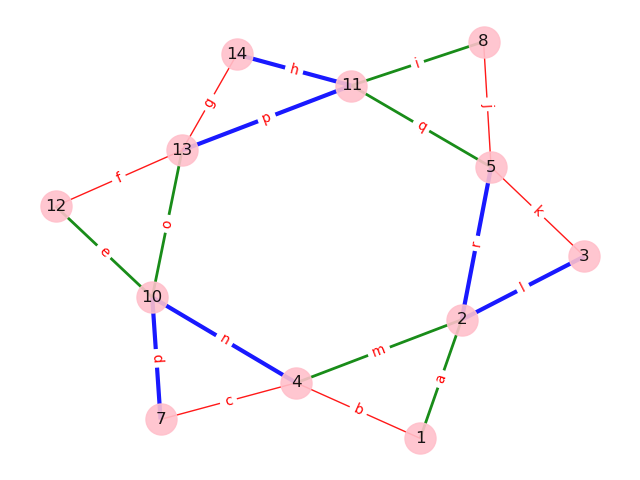
\includegraphics[width=120mm]{img/kagome_double_dimer.png}
\caption{Kagome unit cell with edge colors showing the splitting into three double-dimer configurations.\label{fig:kagome-dd}}
\end{figure}
These are nine double-dimer Hamiltonians
\begin{equation}
\begin{split}
\xgt\xgt\igt + \igt\xgt\xgt +
\ygt\ygt\igt + \igt\ygt\ygt +
\zgt\zgt\igt + \igt\zgt\zgt \\
= \begin{pmatrix}
   2 & 0 & 0 & 0 & 0 & 0 & 0 & 0 \\
 0 & 0 & 2 & 0 & 0 & 0 & 0 & 0 \\
 0 & 2 & -2 & 0 & 2 & 0 & 0 & 0 \\
 0 & 0 & 0 & 0 & 0 & 2 & 0 & 0 \\
 0 & 0 & 2 & 0 & 0 & 0 & 0 & 0 \\
 0 & 0 & 0 & 2 & 0 & -2 & 2 & 0 \\
 0 & 0 & 0 & 0 & 0 & 2 & 0 & 0 \\
 0 & 0 & 0 & 0 & 0 & 0 & 0 & 2 
  \end{pmatrix}
\end{split}
\end{equation}
which have the minimal eigenvalue $-4$ with the two linearly independent eigenvectors
\begin{subequations}\begin{align}
\ket{\psi_{DD1}} &= \frac{1}{\sqrt{6}}
\left(2 \ket{101} - \ket{011} - \ket{110}\right) \\
\ket{\psi_{DD2}} &= \frac{1}{\sqrt{6}}
\left(2 \ket{010} - \ket{100} - \ket{001}\right) \,.
\end{align}\end{subequations}
The former eigenvector can be prepared with the circuit
\begin{equation}
U_{DD1}^{(i,j,k)} = \qquad \begin{array}{c}
\Qcircuit @C=.5em @R=0.2em @!R {
\lstick{i} & \qw & \qw & \gate{\mathrm{H}} & \gate{\mathrm{X}} & \ctrl{2} & \qw  \\
\lstick{j} & \gate{\mathrm{R_Y}(\mathrm{arccos}\tfrac13)} & \gate{\mathrm{Z}} & \ctrl{-1} & \qw & \ctrl{1} & \qw \\
\lstick{k} & \gate{\mathrm{X}} & \qw & \qw & \qw & \gate{\mathrm{X}} & \qw 
}\end{array}
\end{equation}
a transpiled version of which, in terms of hardware gates, is given in appendix~\ref{app:double-dimer-circ}. The state $\ket{\psi_{DD2}}$ is obtained by attaching an X to each qubit:
\begin{equation}
U_{DD2}^{(i,j,k)} = \qquad \begin{array}{c}
\Qcircuit @C=.5em @R=0.2em @!R {
\lstick{i} & \multigate{2}{U_{DD1}^{(i,j,k)}} & \gate{\mathrm{X}} & \qw \\
\lstick{j} & \ghost{U_{DD1}^{(i,j,k)}} & \gate{\mathrm{X}} & \qw \\
\lstick{k} & \ghost{U_{DD1}^{(i,j,k)}} & \gate{\mathrm{X}} & \qw
}\end{array}
\end{equation}
Moreover, we can create a superposition by simply attaching $\ry$ gates:
\begin{equation}
\cos(\tfrac\alpha2) \ket{\psi_{DD1}} + \sin(\tfrac\alpha2) \ket{\psi_{DD2}}
\simeq U_{DD3}^{(i,j,k)} = \qquad \begin{array}{c}
\Qcircuit @C=.5em @R=0.2em @!R {
\lstick{i} & \multigate{2}{U_{DD1}^{(i,j,k)}} & \gate{\mathrm{\ry}(\alpha)} & \qw \\
\lstick{j} & \ghost{U_{DD1}^{(i,j,k)}} & \gate{\mathrm{\ry}(\alpha)} & \qw \\
\lstick{k} & \ghost{U_{DD1}^{(i,j,k)}} & \gate{\mathrm{\ry}(\alpha)} & \qw
}\end{array}
\end{equation}

As for the trimer state above, the full (12+4)-qubit ground state of $H_E$ is then obtained as the product ($\alpha \in \{1,2,3\}$)
\begin{equation}
\ket{\Psi_{DD\alpha}} = U_{DD\alpha} \ket{0}^{\otimes 16}
= U_{DD\alpha}^{(1,4,7)} U_{DD\alpha}^{(3,5,8)} U_{DD\alpha}^{(12,13,14)} \ket{0}^{\otimes 16}
\end{equation}
with the unitaries for the evolution with $H_{E,F,G}$ given by
{\allowdisplaybreaks\begin{subequations}\begin{align}\label{eqn:dd-unitaries}
U_{E}(\vec\theta_{E}) &= \qquad \begin{array}{c}
\Qcircuit @C=.5em @R=0.2em @!R {
\lstick{2} & \qw & \qw & \qw \\
\lstick{1} & \multigate{1}{U_H} & \qw & \qw \\
\lstick{4} & \ghost{U_H} & \multigate{1}{U_H} & \qw \\
\lstick{7} & \qw & \ghost{U_H} & \qw \\
\lstick{10} & \qw & \qw & \qw \\
\lstick{12} & \multigate{1}{U_H} & \qw & \qw \\
\lstick{13} & \ghost{U_H} & \multigate{1}{U_H} & \qw \\
\lstick{14} & \qw & \ghost{U_H} & \qw \\
\lstick{11} & \qw & \qw & \qw \\
\lstick{8} & \multigate{1}{U_H} & \qw & \qw \\
\lstick{5} & \ghost{U_H} & \multigate{1}{U_H} & \qw \\
\lstick{3} & \qw & \ghost{U_H} & \qw 
}\end{array}\\[10pt]
U_{F}(\vec\theta_{F}) &= \qquad \begin{array}{c}
\Qcircuit @C=.5em @R=0.2em @!R {
\lstick{2} & \multigate{1}{U_H} & \qw & \multigate{1}{U_H} & \qw & \qw \\
\lstick{1} & \ghost{U_H} & \qswap & \ghost{U_H} & \qswap & \qw \\
\lstick{4} & \qw & \qswap\qwx & \qw & \qswap\qwx & \qw \\
\lstick{7} & \qw & \qw & \qw & \qw & \qw \\
\lstick{10} & \multigate{1}{U_H} & \qw & \multigate{1}{U_H} & \qw & \qw \\
\lstick{12} & \ghost{U_H} & \qswap & \ghost{U_H} & \qswap & \qw \\
\lstick{13} & \qw & \qswap\qwx & \qw & \qswap\qwx & \qw \\
\lstick{14} & \qw & \qw & \qw & \qw & \qw \\
\lstick{11} & \multigate{1}{U_H} & \qw & \multigate{1}{U_H} & \qw & \qw \\
\lstick{8} & \ghost{U_H} & \qswap & \ghost{U_H} & \qswap & \qw \\
\lstick{5} & \qw & \qswap\qwx & \qw & \qswap\qwx & \qw \\
\lstick{3} & \qw & \qw & \qw & \qw & \qw 
}\end{array}\\[10pt]
U_{G}(\vec\theta_{G}) &= \qquad \begin{array}{c}
\Qcircuit @C=.5em @R=0.2em @!R {
\lstick{5} & \qw & \qswap & \qw & \qswap & \qw \\
\lstick{3} & \multigate{1}{U_H} & \qswap\qwx & \multigate{1}{U_H} & \qswap\qwx & \qw \\
\lstick{2} & \ghost{U_H} & \qw & \ghost{U_H} & \qw & \qw \\
\lstick{1} & \qw & \qw & \qw & \qw & \qw \\
\lstick{4} & \qw & \qswap & \qw & \qswap & \qw \\
\lstick{7} & \multigate{1}{U_H} & \qswap\qwx & \multigate{1}{U_H} & \qswap\qwx & \qw \\
\lstick{10} & \ghost{U_H} & \qw & \ghost{U_H} & \qw & \qw \\
\lstick{12} & \qw & \qw & \qw & \qw & \qw \\
\lstick{13} & \qw & \qswap & \qw & \qswap & \qw \\
\lstick{14} & \multigate{1}{U_H} & \qswap\qwx & \multigate{1}{U_H} & \qswap\qwx & \qw \\
\lstick{11} & \ghost{U_H} & \qw & \ghost{U_H} & \qw & \qw \\
\lstick{8} & \qw & \qw & \qw & \qw & \qw 
}\end{array}
\end{align}\end{subequations}}



\section{Hamiltonian Variational Ansatz (HVA)}\label{sec:hva}
Knowing the ground state $\ket{\Psi_1}$ of $H_1$ we introduce
\begin{equation}
 H(t) = H_1 + t (H_2 + H_3 + H_4)
= (1-t) H_1 + t H
\end{equation}
The adiabatic theorem states that if we evolve $H$ from $H(0) = H_1$ to $H(1) = H$ slowly, the system state remains in the ground state. The unitary evolution with $H(t)$ can be approximated by $\tilde{p}$ steps of times $t_i$ such that $\sum_i t_i = 1$ with the Hamiltonian $H(T_i)$ at the middle time point
\begin{equation}
 T_i = \sum_{j=1}^{i-1} t_j + \frac{t_i}{2}
\end{equation}
Hence, starting from the dimer ground state in subsection~\ref{sec:dimer}, the circuit
\begin{align}\label{eqn:hva-derivation}
 U_\text{HVA} &= \left(\prod_{j=1}^{\tilde{p}} 
\rme^{-\rmi t_j H(T_j)}
\right) U_D \nnl
&\approx \left(\prod_{j=1}^{\tilde{p}} \prod_{k=1}^q 
\rme^{-\rmi \frac{t_j}{q} H_1}
\rme^{-\rmi \frac{t_j}{q} T_j H_2}
\rme^{-\rmi \frac{t_j}{q} T_j H_3}
\rme^{-\rmi \frac{t_j}{q} T_j H_4}
\right) U_D \nnl
&= \left(\prod_{j=1}^{p}
U_H^1(\vec \theta_1)
U_H^2(\vec \theta_2)
U_H^3(\vec \theta_3)
U_H^4(\vec \theta_4)
\right) U_D
\end{align}
should prepare the ground state of $H$ for sufficiently large $p = \tilde{p}q$, where we trotterized from the first to the second line. The equality of the last line holds if $\vec \theta_1 = (t_j/q) \vec{1}$ and $\vec \theta_{2,3,4} = (t_j/q) T_j \vec{1}$ for the corresponding $j$, which, therefore, is a good choice for the initial VQE parameters.

However, for the purpose of the VQE we leave the $\vec\theta_{1,2,3,4}$ as free variational parameters. Furthermore, instead of keeping the same parameters for each Trotter step, we choose different parameters $\vec\theta_{1,2,3,4}^j$ (with entries in $[0,1]$) for every step, resulting in a total number of $54 p$ parameters and the ansatz
\begin{equation}\label{eqn:hva-dimer}
 U_\text{HVA}
= \left(\prod_{j=1}^{p}
U_H^1(\vec \theta_1^j)
U_H^2(\vec \theta_2^j)
U_H^3(\vec \theta_3^j)
U_H^4(\vec \theta_4^j)
\right) U_D
\end{equation}
Assuming equal time steps $t_i \equiv 1/\tilde{p}$, and $\tilde{p}=q=\sqrt{p}$, the initial values according to equation~\eqref{eqn:hva-derivation} are
\begin{equation}
\vec\theta_1^j = \frac{\vec{1}}{p} \qquad\text{and}\qquad
\vec\theta_{2,3,4}^j = \frac{\vec{1}}{p\sqrt{p}} \left(\left\lfloor\frac{j}{\sqrt{p}}\right\rfloor - \frac{1}{2}\right) \,.
\end{equation}

In complete analogy, the HVA ansatz starting from the trimer ground state found in subsection~\ref{sec:trimer} is given by
\begin{equation}\label{eqn:hva-trimer}
 U_\text{HVA}^\alpha
= \left(\prod_{j=1}^{p}
U_A(\vec \theta_A^j)
U_B(\vec \theta_B^j)
\right) U_{T\alpha}
\end{equation}
where $\alpha$ labels the selected initial state and each $\vec\theta_{A,B}^j$ is a vector of 27 parameters amounting, again, to a total of $54p$ parameters, initialized with
\begin{equation}\label{eqn:hva-trimer-initial-parameters}
\vec\theta_A^j = \frac{\vec{1}}{p} \qquad\text{and}\qquad
\vec\theta_B^j = \frac{\vec{1}}{p\sqrt{p}} \left(\left\lfloor\frac{j}{\sqrt{p}}\right\rfloor - \frac{1}{2}\right) \,.
\end{equation}

\section{Degenerate subspace optimization}
The basic idea is that, since the Hamiltonian $H$ has a degenerate ground state, we search for a 2-dimensional subspace rather than a single ground state, and then continue by searching the state with minimal energy on this subspace.

In terms of real vector spaces, this can be motivated as follows: Assume the eigenspace to the lowest eigenvalue is spanned by the normalized orthogonal vectors $\vec v_{1,2} \in \R^n$ with $\vec v_1 \cdot \vec v_2 = 0$, such that for any given $a \in [0,1]$
\begin{equation}
 \vec v = a \vec v_1 + \sqrt{1-a^2} \vec v_2
\end{equation}
is a normalized eigenvector to the lowest eigenvalue. Now say our algorithm finds orthogonal vectors $\vec w_{1,2} \in \R^n$ close to $\vec v_{1,2}$, respectively, i.e. with
\begin{subequations}\begin{align}
\vec v_1 \cdot \vec w_1 
= \vec v_2 \cdot \vec w_2
&= 1 - \varepsilon \\
\vec v_1 \cdot \vec w_2 
= \vec v_2 \cdot \vec w_1
&= \varepsilon
\end{align}\end{subequations}
Then we have for
\begin{equation}
 \vec w = a \vec w_1 + \sqrt{1-a^2} \vec w_2
\end{equation}
that the overlap with the exact eigenstate $\vec v$ is
\begin{equation}
\vec v \cdot \vec w = 1 - \varepsilon \left(1 - 2 a \sqrt{1-a^2}\right)
\end{equation}
which reaches a maximum value of 1 for $a = 1/\sqrt{2}$.

Hence, wheras $\vec w_1$ and $\vec w_2$ are both only approximately in the eigenspace with an error of $\varepsilon$, there exists a vector $\vec w$ in the span of both vectors that overlaps exactly with an eigenvector $\vec v$. Although in practical situations the two vectors $\vec w_{1,2}$ will not be related to the pair $\vec v_{1,2}$ by a simple rotation as in this example, intuition suggests that there are still vectors in the subspace spanned by $\vec w_1$ and $\vec w_2$ which are closer to a ground state than either of these vectors.

In a complex vector space, the superposition will depend on three real parameters (global and relative phase, as well as one magnitude, with the other determined by the normalization constraint). Finding the optimal state in the two dimensional subspace is then an optimization problem with three real parameters and should show much better convergence with much less severe barren plateau issues. As we will see below, in practice we can only search a one-parameter subspace of the full three-parameter space.

\subsection{Cost function}
In order to apply this to our VQE problem, we start with the orthogonal initial trimer eigenstates $\ket{\Psi_{T1}}$ and $\ket{\Psi_{T2}}$ for our HVA ansatz. Since unitary evolution conserves orthogonality, the resulting ansatz states 
\begin{equation}
\ket{\Psi_{1,2}(\vec\theta)} = U_\text{HVA}^{1,2}(\vec\theta) \ket{0}^{\otimes n}
\end{equation}
will be orthogonal, as long as we evolve them with the \emph{same} parameters $\vec\theta$.

In order to find the degenerate subspace, we therefore optimize the cost function
\begin{equation}\label{eqn:cost-function}
 C(\vec\theta) = \bra{\Psi_1(\vec\theta)} H \ket{\Psi_1(\vec\theta)} + \bra{\Psi_2(\vec\theta)} H \ket{\Psi_2(\vec\theta)}
\end{equation}




\subsection{Superposition states via circuit}

In principle, we can create a single qubit superposition state as
\begin{equation}
\cos\tfrac\alpha2 \ket{0} + \rme^{\rmi \beta}\sin\tfrac\alpha2 \ket{1} = \pgt(\beta)\ry(\alpha)\ket{0}
\end{equation}
Thus, for any two $n$-qubit states $\ket{\Psi_{1,2}} = U_{1,2} \ket{0}^{\otimes n}$ we can prepare a superposition $\cos\tfrac\alpha2 \ket{\Psi_1} + \rme^{\rmi \beta}\sin\tfrac\alpha2 \ket{\Psi_2}$ via an auxiliary qubit:
\begin{equation}\label{eqn:superpos-circuit}
U_\text{SUP}(\alpha,\beta) = \qquad
\begin{array}{c}
\Qcircuit @C=.5em @R=0.2em @!R {
\lstick{\text{aux}} & \gate{\ry(\alpha)} & \gate{\pgt(\beta)} & \ctrl{1} & \gate{\xgt} & \ctrl{1} & \gate{\xgt} & \qw \\
\lstick{1} & \qw & \qw & \multigate{2}{U_2} & \qw & \multigate{2}{U_1} & \qw & \qw \\
& \cdots & & \nghost{U_2} &  & \nghost{U_1} &  & \cdots  \\
\lstick{n} & \qw & \qw & \ghost{U_2} & \qw & \ghost{U_1} & \qw & \qw
}\end{array}
\end{equation}
Precisely speaking, this circuit prepares the entangled $n+1$ qubit state $\cos\tfrac\alpha2 \ket{0}_0 \otimes \ket{\Psi_1}_{1,\dots,n} + \rme^{\rmi \beta}\sin\tfrac\alpha2 \ket{1}_0 \otimes \ket{\Psi_2}_{1,\dots,n}$, which amounts to a superposition for operators acting only on the qubits $1,\dots,n$.
However, creating the controlled gates $U_{1,2}$ will generally require a circuit of large depth.

For the circuits $U_{T1}$ and $U_{T2}$ as defined in equations~\eqref{eqn:circ-ut1} and~\eqref{eqn:circ-ut2}, we can construct a circuit of depth 117 matched to the Guadalupe layout, as shown in appendix~\ref{app:superpos-of-trimers}. The full 16-qubit circut representing the superposition is given by three parallel copies of this circuit for the qubits $(\text{aux},i,j,k) \in \{(0,2,1,4),(15,10,12,13),(9,11,8,5)\}$, respectively. That is, we use the adjacent qubits 0, 15, and 9 for each of the three trimer terms, with the same parameters $\alpha$ and $\beta$. We must then post-select for measurements where these three qubits have the same value. We also omit the final $\xgt$ on the auxiliary qubit and swap the circuits setting $U_1 = U_{T2}$ and $U_2 = U_{T1}$ in equation~\eqref{eqn:superpos-circuit} which results in a shorter circuit.
The prepared state is then
\begin{equation}
\ket{\Psi_\text{SUP}} =
\left(\rme^{\rmi \beta} \sin\tfrac\alpha2 \ket{0}_\text{aux} \otimes \ket{\psi_{T1}}_{i,j,k} + \cos\tfrac\alpha2 \ket{1}_\text{aux} \otimes \ket{\psi_{T2}}_{i,j,k} \right)^{\otimes 3} \,.
\end{equation}
Hence, measuring $q_0 = q_{15} = q_9 = 0$ corresponds to finding the system in the initial state $\ket{\Psi_{T1}}$ and measuring $q_0 = q_{15} = q_9 = 1$ to $\ket{\Psi_{T2}}$.

Using this superposition state as the initial state in our HVA ansatz~\eqref{eqn:hva-trimer} results in the ansatz
\begin{equation}\label{eqn:hva-superpos}
 U_\text{HVA}^\text{SUP}
= \left(\prod_{j=1}^{p}
U_A(\vec \theta_A^j)
U_B(\vec \theta_B^j)
\right) U_\text{SUP}
\end{equation}
which uses 15 active qubits, has two more parameters, $\alpha$ and $\beta$, totalling to $54p + 2$ parameters, and a circuit depth of $102p + 117$.

We can either optimize the ansatz~\eqref{eqn:hva-superpos} independently, or use the parameters $\vec\theta_\text{min}$ obtained by minimizing the cost function~\eqref{eqn:cost-function} as fixed parameters and only optimize~\eqref{eqn:hva-superpos} over the $(\alpha,\beta)$ parameter space.


\subsection{Superpositions in classical computation}
Given $m$ approximated ground states $\ket{\Psi_i} = U_i \ket{0}^{\otimes n}$---i.e. given optimized parameter vectors $\vec{\theta}_i$ for the circuits $U_i$ (which can be different from each other or the same)---we can calculate the matrix elements
\begin{equation}
 H_{ij} = \bra{\Psi_i} H \ket{\Psi_j}
 = \rme^{\rmi \varphi_{ij}} h_{ij}
\end{equation}
with $h_{ij}, \varphi_{ij} \in \R$, $h_{ij} = h_{ji}$, and $\varphi_{ij} + \varphi_{ji} = 0$, specifically $\varphi_{ii} = 0$.

For a generic superposition state
\begin{equation}
 \ket{\Psi} = \sum_{i=1}^m \alpha_i \rme^{\rmi \beta_i} \ket{\Psi_i}
\end{equation}
with $\vec\alpha, \vec\beta \in \R^m$ and normalization constraint $\sum_{i=1}^m \alpha_i^2 = 1$, we find
\begin{equation}
 \bra{\Psi} H \ket{\Psi} 
 = \sum_{i=1}^m \sum_{j=1}^m \alpha_i \alpha_j \rme^{\rmi(\beta_j-\beta_i)} H_{ij}
 = \sum_{i=1}^m \sum_{j=1}^m \alpha_i \alpha_j \rme^{\rmi(\beta_j-\beta_i+\varphi_{ij})} h_{ij}
\end{equation}
Generally, we cannot calculate this expression, as we only have access to $h_{ij}$ via measurements, and not the phases $\varphi_{ij}$. For $m \leq 3$, however, we can absorb the $m(m-1)/2$ nontrivial phases by the choice of the $m$ parameters $\beta_i$ (restricting the subspace spanned by the superposition states).

Specifically, for $m=3$ we have
\begin{align}
 \bra{\Psi} H \ket{\Psi} 
 &= \alpha_1^2 (h_{11}-h_{33})
 + \alpha_2^2 (h_{22}-h_{33})
 + h_{33} \nnl
&\bleq + 2 \alpha_1 \alpha_2 h_{12}
+ 2 \sqrt{1-\alpha_1^2-\alpha_2^2} \left( \alpha_1 h_{13}
+ \alpha_2 h_{23} \right)
\end{align}
with free parameters $\alpha_{1,2}$, and for $m=2$ we have
\begin{align}\label{eqn:matrix-elem-m2}
 \bra{\Psi} H \ket{\Psi} 
 &= \alpha^2 (h_{11}-h_{22}) + h_{22}
 + 2 \alpha \sqrt{1-\alpha^2} h_{12}
\end{align}
which depends only on the free parameter $\alpha = \alpha_1$ and is independent of the remaining relative global phase (the relative phase is fixed by $\varphi_{12} = \beta_2-\beta_1$).
Equation~\eqref{eqn:matrix-elem-m2} has four local extrema (for $\sigma, \tau \in \{\pm 1\}$):
\begin{equation}
\alpha^\text{min} = \pm \frac{1}{\sqrt{2}}\left(1 \pm \left(1 + \left(\frac{2h_{12}}{h_{11} - h_{22}} \right)^2\right)^{-1/2}\right)^{1/2} \,,
\end{equation}
resulting in the minimal eigenvalue
\begin{equation}\label{eqn:hmin-subspace}
 \ev{H}_\text{min} 
 = \frac{1}{2} \left(h_{11} + h_{22} 
 - \sqrt{(h_{11} - h_{22})^2 + 4 h_{12}^2}\right) \,.
\end{equation}
If $h_{12} = 0$, this is simply the smaller of $h_{11}$ and $h_{22}$, becoming the smaller, the larger $\abs{h_{12}}$.


Whereas the expectation values are easily measured, the off-diagonal matrix element $h_{12}$ is not. Considering that $\ket{\Psi_{1,2}}$ are orthogonal, we can however write
\begin{align} \label{eqn:h12-estimate}
h_{12}
 &= \abs{\bra{\Psi_1} H \ket{\Psi_2}} \nnl 
 &=
 \abs{\bra{\Psi_1} \rmi \rme^{\rmi H t} \frac{\partial}{\partial t}\rme^{-\rmi H t}  \ket{\Psi_2}} \nnl
 &= \abs{\bra{\Psi_1} \frac{\rmi}{\varepsilon} \left(\rme^{-\rmi H \varepsilon} - 1 - \frac{\varepsilon^2}{2} \frac{\partial^2}{\partial \delta^2}\rme^{-\rmi H \delta} \right)  \ket{\Psi_2}} \nnl
 &= \abs{\frac{1}{\varepsilon} \bra{\Psi_1} \rme^{-\rmi H \varepsilon} \ket{\Psi_2} + \frac{\varepsilon}{2} \bra{\Psi_1} H^2\rme^{-\rmi H \delta} \ket{\Psi_2}} \nnl
 &\geq \frac{1}{\varepsilon} \abs{\bra{\Psi_1} \rme^{-\rmi H \varepsilon} \ket{\Psi_2}} - \frac{\varepsilon}{2}\abs{\bra{\Psi_1} H^2\rme^{-\rmi H \delta} \ket{\Psi_2}} \nnl
 &\geq \frac{1}{\varepsilon} \abs{\bra{\Psi_1} \rme^{-\rmi H \varepsilon} \ket{\Psi_2}} - \frac{\varepsilon}{2}\norm{ H^2\rme^{-\rmi H \delta} } \nnl
&\geq \frac{1}{\varepsilon} \abs{\bra{\Psi_1} \rme^{-\rmi H \varepsilon} \ket{\Psi_2}} - \frac{\varepsilon}{2}\norm{H}^2 \nnl
&= \frac{1}{\varepsilon} \abs{\bra{\Psi_1} \rme^{-\rmi H \varepsilon} \ket{\Psi_2}} - \frac{\varepsilon}{2} 18^2 \,,
\end{align}
where in the third line we evaluate the (time independent) expression at $t=0$ and use first order Taylor expansion with remainder in Lagrange form for some $\delta \in [0,\varepsilon]$. In the fourth line we make use of the orthogonality $\braket{\Psi_1}{\Psi_2} = 0$.

We can then trotterize the exponential to second order
\begin{equation}
U_T(\varepsilon) = U_Z(\varepsilon \vec{1}) U_Y(\varepsilon \vec{1}) U_X(\varepsilon \vec{1}) U_X(\varepsilon \vec{1})
U_Y(\varepsilon \vec{1}) U_Z(\varepsilon \vec{1})
\end{equation}
where we use the term grouping with the smallest number of mutually commuting clusters into $U_{X,Y,Z}$, where there ordering is chosen to minimize the circuit depth.
This circuit has the error bound~\cite{childsTheoryTrotterError2021}
\begin{equation}
\norm{U_T(\varepsilon) - \rme^{-\rmi H \varepsilon}} 
\leq \frac{\varepsilon^3}{24} (2 L_X + 2 L_Y + M_X + M_Y)
\end{equation}
where
\begin{align}
 L_X &= \norm{\comm{\comm{H_X}{H_Y+H_Z}}{H_Y+H_Z}} \nnl
&\leq \norm{\comm{H_Y}{\comm{H_X}{H_Y}}} +
\norm{\comm{H_Y}{\comm{H_X}{H_Z}}} \nnl &\bleq +
\norm{\comm{H_Z}{\comm{H_X}{H_Y}}} +
\norm{\comm{H_Z}{\comm{H_X}{H_Z}}}  \nnl
 L_Y &= \norm{\comm{H_Z}{\comm{H_Y}{H_Z}}} \nnl
 M_X &= \norm{\comm{H_X}{\comm{H_X}{H_Y+H_Z}}} \nnl
&\leq \norm{\comm{H_X}{\comm{H_X}{H_Y}}} +
\norm{\comm{H_X}{\comm{H_X}{H_Z}}} \nnl
 M_Y &= \norm{\comm{H_Y}{\comm{H_Y}{H_Z}}}
\end{align}
and $\norm{A}$ denotes the spectral norm of $A$ (i.e. $\sqrt{\lambda}$ where $\lambda$ is the largest eigenvalue if $A^\dagger A$). Hence, writing
\begin{equation}
 N_{\rho\sigma\tau} = \norm{\comm{H_\rho}{\comm{H_\sigma}{H_\tau}}}
\end{equation}
we have
\begin{align}\label{eqn:trotter-error-bound}
\norm{U_T(\varepsilon) - \rme^{-\rmi H \varepsilon}} 
&\leq \frac{\varepsilon^3}{24} (2 N_{YXY} + 2 N_{YXZ} + 2 N_{ZXY} + 2 N_{ZXZ} \nnl
&\bleq + 2 N_{ZYZ} + N_{XXY} + N_{XXZ} + N_{YYZ}) \nnl
&\approx 283 \varepsilon^3
\end{align}
With the trotterized circuit
\begin{equation}\label{eqn:uoff-circuit}
 U_\text{off}(\varepsilon,\vec\theta) = U_\text{HVA}^{1\dagger}(\vec\theta) U_T(\varepsilon) U_\text{HVA}^{2}(\vec\theta)
\end{equation}
evaluated at the parameters $\vec\theta_\text{min}$ minimizing the cost function~\eqref{eqn:cost-function}, we can obtain
\begin{equation}
P(\varepsilon) = \abs{\bra{0}^{\otimes n} U_\text{off}(\varepsilon,\vec\theta_\text{min}) \ket{0}^{\otimes n}}^2
\end{equation}
by preparing the state $U_\text{off}(\varepsilon,\vec\theta_\text{min}) \ket{0}^{\otimes n}$ and measuring the probability of finding $\ket{0}^{\otimes n}$. We then use the lower bound
\begin{equation}\label{eqn:off-diags}
 h_{12} = \max_\varepsilon\left(\sqrt{\frac{P(\varepsilon)}{\varepsilon^2} - 283 \varepsilon} - 162 \varepsilon\right)
\end{equation}
and, assuming this expression is positive, can obtain an upper bound on the ground state energy via equation~\eqref{eqn:hmin-subspace}.

\paragraph{A note on scalability}
Calculating the norms $N_{\rho\sigma\tau}$ numerically is quite time consuming. A better scalable approach would be to estimate the norms by counting the number of noncommuting Pauli strings involved in the double commutators. These can be easily counted to be 456 for $N_{YXZ}$ and $N_{ZXY}$, and 408 for the remaining six double commutators, where every double commutator adds 4 to the norm (note that the nonzero commutators of two Pauli strings are $2\rmi^k$ times another Pauli string, and all Pauli strings have norm 1), amounting to an upper bound of $916 \varepsilon^3$ instead in equation~\eqref{eqn:trotter-error-bound}. Similarly, we could have used the total number of Pauli strings as a bound on $\norm{H} \leq 54$ in equation~\eqref{eqn:h12-estimate} for better scalability.

\paragraph{Accuracy of the limit}
All inequalities given in this section are, in principle, precise. Thus, in theory, $\ev{H}_\text{min}$ obtained according to equation~\eqref{eqn:hmin-subspace} is guaranteed not to become smaller than the exact value. A measurement error resulting in a too large value $P(\varepsilon)$ could nonetheless result in a value of $\ev{H}_\text{min}$ below the exact one. This is, however, not different from the standard VQE algorithm, which possesses the exact ground state energy as a theoretical bound but could fall below it by coincidence due to measurement errors on single operators adding up.
\warning{A crucial difference is that noise is typically expected to drive the states $\ket{\Psi_{1,2}}$ away from a ground state, which for the variational principle implies that it increases the expectation value. For the off-diagonal $h_{12}$ here, the same noise would result in a larger $P(\varepsilon)$ for small $\varepsilon$ and, thus, increase $h_{12}$, i.e. decrease the ground state energy, potentially below its exact value.}




\section{Measuring the matrix elements}\label{sec:measuring}
In order to obtain the expectation value
\begin{equation}
H_{\alpha\alpha} = \bra{\Psi_\alpha} H \ket{\Psi_\alpha} 
= \bra{0} U_\text{HVA}^\alpha{}^\dagger H U_\text{HVA}^\alpha \ket{0}
\end{equation}
we can use Qiskit Runtime estimator. First we load Qiskit Runtime with options. Note that we choose to skip transpilation, assuming that the ansatz circuits are already optimized using hardware gates.
\begin{python}
from qiskit_ibm_runtime import QiskitRuntimeService,
     Session, Estimator, Sampler, Options
from qiskit.providers.fake_provider import FakeGuadalupeV2
from qiskit_aer.noise import NoiseModel

# Load Qiskit Runtime Service
service = QiskitRuntimeService(channel='ibm_quantum')

# For simulator use FakeGuadalupe as model:
fake_backend = FakeGuadalupeV2()
noise_model  = NoiseModel.from_backend(fake_backend)
coupling_map = fake_backend.coupling_map
basis_gates  = fake_backend.operation_names
options = Options(simulator={'noise_model':  noise_model,
                             'coupling_map': coupling_map,
                             'basis_gates':  basis_gates}, 
                  transpilation={'skip_transpilation': True})

# Select the backend
backend = service.backends(simulator=True)[0]
\end{python}
%
The Hamiltonian can be defined from a list of edges of the Kagome lattice, taking care of the correct assignment of vertices to physical qubits:
\begin{python}
from qiskit.quantum_info import SparsePauliOp
from qiskit.opflow.primitive_ops import PauliSumOp

num_qubits = 16

# every edge in the Kagome lattice contributes three Pauli
# strings with X/Y/Z on the corresponding vertices:
kagome_edges = [(2,1),(1,4),(4,7),(7,10),(10,12),(12,13),
                (13,14),(14,11),(11,8),(8,5),(5,3),(3,2),
                (2,4),(4,10),(10,13),(13,11),(11,5),(5,2)]
    
# Construct the hamiltonians for the estimator
pauli_strings = {'X': [], 'Y': [], 'Z': []}
for e in kagome_edges:
    for c in 'XYZ':
        s = ''
        for i in range(num_qubits):
            if i in e:
                s = c + s
            else:
                s = 'I' + s
        pauli_strings[c].append(s)
hamiltonian = PauliSumOp(SparsePauliOp(pauli_strings['X']
              +pauli_strings['Y']+pauli_strings['Z']))
\end{python}
%
The routine to estimate the expectation value is then given by:
\begin{python}
def expectation_value(hamiltonian, ansatz, parameters):
    with Session(service=service, backend=backend):
        estimator = Estimator(options=options)
        job = estimator.run(circuits=[ansatz],
              parameter_values=[parameters],
              observables=[hamiltonian])
        res = job.result()
    ev = res.values[0]
    return ev
\end{python}
where \pyth{ansatz} is the ansatz circuit $U_\text{HVA}$ as defined in equations~\eqref{eqn:hva-dimer} for the dimer, \eqref{eqn:hva-trimer} for the trimer ground state, and \eqref{eqn:hva-superpos} for the superposition, respectively, and \pyth{ansatz_parameters} the vector $\vec\theta$ parameterizing this circuit.

\subsection{Measuring a Pauli string}
Note that we can represent any hermitian operator $H$ in terms of its orthonormal eigenbasis:
\begin{equation}
H = \sum_i h_i \ket{h_i}\bra{h_i}
\end{equation}
Let $B$ be the unitary basis transformation to the computational basis, i.e. $\ket{i} = B \ket{h_i}$. Then we have
\begin{equation}
 \widetilde{H} = B H B^\dagger
 = \sum_i h_i B \ket{h_i} \bra{h_i} B^\dagger
 = \sum_i h_i \ket{i} \bra{i}
\end{equation}
diagonal in the computational basis.
For an ansatz state $\ket{\psi} = U \ket{0}$ with some unitary $U$, we then have
\begin{align}
\bra{\psi} H \ket{\psi}
&= \bra{\psi} B^\dagger \widetilde{H} B \ket{\psi} \nnl
&= \sum_i h_i \bra{0} U^\dagger B^\dagger  \ket{i}\bra{i} B U \ket{0} \nnl
&= \sum_i h_i \abs{\bra{i} B U \ket{0}}^2 \nnl 
&= \sum_i h_i P_i(B \ket{\psi})
\end{align}
where $P_i(B \ket{\psi})$ is the probability to measure $\ket{i}$ in the prepared state $B \ket{\psi}$.

Writing the single-qubit Pauli operators as $\sigma_0 = \igt$, $\sigma_1 = \xgt$, $\sigma_2 = \ygt$, $\sigma_3 = \zgt$, we can define $n$-qubit Pauli strings by vectors $\vec\mu \in \{0,1,2,3\}^n$:
\begin{equation}
H_{\vec\mu} = \prod_{i=0}^{n-1} \sigma_{\mu_i}^{(i)}
\qquad \text{with} \quad
\mu_i \in \{0,1,2,3\} \,.
\end{equation}
$H_{\vec\mu}$ is diagonal in the basis
\begin{equation}
\ket{\widetilde{s}} = \bigotimes_{i=0}^{n-1} \ket{(s_i)_{\mu_i}}
\end{equation}
where $s \in \{0,1,\dots,2^n-1\}$, $s_i \in \{0,1\}$ denotes the value of the $i$-th bit of $s$ in binary form, and we have
\begin{equation}\begin{aligned}
\ket{0_1} &= \ket{+} = \frac{1}{\sqrt{2}}\left(\ket{0}+\ket{1}\right) \,,\qquad& \ket{1_1} &= \ket{-} = \frac{1}{\sqrt{2}}\left(\ket{0}-\ket{1}\right) \\
\ket{0_2} &= \ket{y_+} = \frac{1}{\sqrt{2}}\left(\ket{0}+\rmi\ket{1}\right) \,,\qquad& \ket{1_2} &= \ket{y_-} = \frac{1}{\sqrt{2}}\left(\ket{0}-\rmi\ket{1}\right) \\
\ket{0_3} &= \ket{0_0}  = \ket{0} \,,\qquad& \ket{1_3} &= \ket{1_0} = \ket{1} 
\end{aligned}\end{equation}
The corresponding eigenvalues $H_{\vec\mu} \ket{\widetilde{s}} = h_{\vec\mu} \ket{\widetilde{s}}$ are
\begin{align}\label{eqn:pauli-string-eigenvalues}
h_{\vec\mu} &= \prod_{i=0}^{n-1} (-1)^{r_i s_i}  = \pm 1 \,,
\intertext{where}
r_i &= 1 - 0^{\mu_i} = \begin{cases}0 &\quad\text{for } \sigma^{(i)} = \igt_i \\ 1 &\quad\text{for } \sigma^{(i)} \in \{\xgt_i, \ygt_i, \zgt_i\} \end{cases}
\end{align}
i.e. each $\xgt_i$, $\ygt_i$, or $\zgt_i$ contributes a factor of $-1$ if the corresponding bit $s_i = 1$, wheras all qubits with either an $\igt_i$ (and therefore $\mu_i=0$) in the Pauli string or a bit $s_i = 0$ in the state contribute a factor of $1$.


For single qubits $s_i \in \{0,1\}$ we have the transformations from the $x$ and $y$ bases to the computational basis 
\begin{align}
\hgt \ket{(s_i)_1} &= \ket{(s_i)_0} \\
\hgt \sdg \ket{(s_i)_2} &= \ket{(s_i)_0}
\end{align}
(Note the difference in notation: $\hgt$ is the Hadamard gate, wheras the Hamiltonian is denoted $H$ in italics.)
The basis transformation $B$ that renders $H_{\vec\mu}$ diagonal in the $n$-qubit computational basis, is then the tensor product
\begin{equation}
 B_{\vec\mu} = \bigotimes_{i=0}^{n-1} B_{\mu_i} \qquad \text{with} \quad
 B_1 = \hgt \,,
 B_2 = \hgt\sdg \,,
 B_3 = B_0 = \igt \,.
\end{equation}
As a circuit, $B_{\vec\mu}$ appends $\Qcircuit @C=.5em @R=0.2em @!R {& \gate{\hgt} & \qw}$ to all qubits where the Pauli string $H_{\vec\mu}$ has an $\xgt$ and $\Qcircuit @C=.5em @R=0.2em @!R {& \gate{\sdg} & \gate{\hgt} & \qw}$ to all qubits where it has a $\ygt$.

Generally, commuting Pauli strings can be measured with the same basis transformation $B$. In our case, where $H = H^X + H^Y + H^Z$ can be split in parts containing only $\igt$ as well as $\xgt$, $\ygt$, or $\zgt$, respectively, we can measure all Pauli strings in $H^{X,Y,Z}$ simultaneously, requiring only three measurements in total with the circuits:
\begin{align}
U^X_\text{meas} &= \quad \begin{array}{c}
\Qcircuit @C=.5em @R=0.2em @!R {
\lstick{0} & \qw & \qw & \qw & \multigate{3}{U_\text{HVA}^\text{SUP}} & \gate{\hgt} & \meter & \qw \\
\lstick{1} & \qw & \qw & \qw & \ghost{U_\text{HVA}^\text{SUP}} & \gate{\hgt} & \meter & \qw \\
& \cdots &  & &  \nghost{U_\text{HVA}^\text{SUP}} & & \cdots  \\
\lstick{15} & \qw & \qw & \qw & \ghost{U_\text{HVA}^\text{SUP}} & \gate{\hgt} & \meter & \qw
}\end{array} \\[10pt]
U^Y_\text{meas} &= \quad \begin{array}{c}
\Qcircuit @C=.5em @R=0.2em @!R {
\lstick{0} & \qw & \qw & \qw & \multigate{3}{U_\text{HVA}^\text{SUP}} & \gate{\sdg} & \gate{\hgt} & \meter & \qw \\
\lstick{1} & \qw & \qw & \qw & \ghost{U_\text{HVA}^\text{SUP}} & \gate{\sdg} & \gate{\hgt} & \meter & \qw \\
& \cdots &  & &  \nghost{U_\text{HVA}^\text{SUP}} & & & \cdots  \\
\lstick{15} & \qw & \qw & \qw & \ghost{U_\text{HVA}^\text{SUP}} & \gate{\sdg} & \gate{\hgt} & \meter & \qw
}\end{array} \\[10pt]
U^Z_\text{meas} &= \quad \begin{array}{c}
\Qcircuit @C=.5em @R=0.2em @!R {
\lstick{0} & \qw & \qw & \qw & \multigate{3}{U_\text{HVA}^\text{SUP}} & \qw & \meter & \qw \\
\lstick{1} & \qw & \qw & \qw & \ghost{U_\text{HVA}^\text{SUP}} & \qw & \meter & \qw \\
& \cdots &  & &  \nghost{U_\text{HVA}^\text{SUP}} & & \cdots  \\
\lstick{15} & \qw & \qw & \qw & \ghost{U_\text{HVA}^\text{SUP}} & \qw & \meter & \qw
}\end{array} 
\end{align}
The measurement results are the probabilities $P^{X,Y,Z}(s)$ for all possible bitstrings $s \in \{0,1,\dots,2^{16}-1\}$.

From the eigenvalues~\eqref{eqn:pauli-string-eigenvalues} we can calculate the weights as the sum over all Kagome edges
\begin{equation}
w_K(s) = \sum_{<i,j> \in \Gamma} (-1)^{s_i + s_j} \,.
\end{equation}
Note that, for the Kagome lattice, all these weights are nonzero.
In order to correctly account for the superposition in our ansatz~\eqref{eqn:hva-superpos}, we must post-select those results with identical values on the auxiliary qubits 0, 9, 15. Therefore, we introduce the modified weight function
\begin{equation}
w_S(s) = \begin{cases}
w_K(s) &\quad \text{if } s_0 = s_9 = s_{15} \\
0 &\quad \text{else}
\end{cases}
\end{equation}
and the cumulative probability of all the disregarded results
\begin{equation}
\overline{P}^{X,Y,Z} = \sum_{\substack{s = 0\\w_S(s) = 0}}^{2^{16}-1} P^{X,Y,Z}(s) \,.
\end{equation}
We then have the expectation value
\begin{equation}
\bra{\psi} H \ket{\psi} = \sum_{\sigma \in \{X,Y,Z\}} \frac{\sum_{s=0}^{2^{16}-1} w_S(s) P^\sigma(s)}{1 - \overline{P}^\sigma}
\end{equation}

The weights $w_S$ are calculated using the following code:
\begin{python}
# set number of qubits and the format string used to turn
# numbers into bitstrings
num_qubits = 16
format_string = '016b' # must match num_qubits

kagome_edges = [(2,1),(1,4),(4,7),(7,10),(10,12),(12,13),
                (13,14),(14,11),(11,8),(8,5),(5,3),(3,2),
                (2,4),(4,10),(10,13),(13,11),(11,5),(5,2)]
aux_qubits = (0,9,15) # these must be all 0 or all 1

# convert the Pauli strings into a bitstring, where the
# position of X/Y/Z is marked by a 1 and I by a 0
ops = list(map(lambda x: 2**x[0]+2**x[1], kagome_edges))

# calculate the weights
weights = []
for i in range(2**num_qubits):
    w = 0
    aux_vals = [i//2**aux%2 for aux in aux_qubits]
    if all(aux_vals) or not any(aux_vals):
        for o in ops:
            s = format(i & o,format_string)
            w += (-1)**(s.count('1'))
    weights.append(w)
\end{python}




\subsection{Superposition states}
In order to use the superposition ansatz~\eqref{eqn:hva-superpos} to optimize the ground state energy over the degenerate subspace, we must condition measurement results on the auxiliary qubits. Hence, we use \pyth{Sampler} rather than \pyth{Estimator}.

\begin{python}
from math import pi

def sampler_expectation_value(weights, ansatz, parameters):
    # Construct circuits for X, Y, Z measurements
    num_qubits = ansatz.num_qubits
    qcX = QuantumCircuit(num_qubits)
    qcY = QuantumCircuit(num_qubits)
    qcZ = QuantumCircuit(num_qubits)
    for qc in [qcX, qcY, qcZ]:
        qc.append(ansatz,range(num_qubits))
    for i in range(num_qubits):
        # Apply Hadamard for rotation to X-basis
        qcX.rz(pi/2,i)
        qcX.sx(i)
        qcX.rz(pi/2,i)
        # Apply H Sdg for rotation to Y-basis
        qcY.sx(i)
        qcY.rz(pi/2,i)
    for qc in [qcX, qcY, qcZ]:
        qc.measure_all()
    # Sample quantum circuits with ansatz parameters:
    with Session(service=service, backend=backend):
        sampler = Sampler(options=options)
        job = sampler.run(circuits=[qcX,qcY,qcZ], 
                          parameter_values=[parameters]*3)
        res = job.result()
    ev = 0
    # sum over the probabilities for X, Y, Z circuit
    for quasi_dist in res.quasi_dists:
        pd = quasi_dist.nearest_probability_distribution()
        ev_part = 0
        p_bar = 0
        for i in pd.keys():
            if weights[i]:
                ev_part += weights[i] * pd[i]
            else:
                p_bar += pd[i]
        ev += ev_part / (1 - p_bar)
    return ev
\end{python}




\subsection{Off-diagonal elements}
In order to use equations~\eqref{eqn:hmin-subspace} and \eqref{eqn:off-diags} to optimize the ground state energy over the degenerate subspace classically, we need to measure $P(\varepsilon)$, i.e. sample the circuit $U_\text{off}$ as defined in equation~\eqref{eqn:uoff-circuit} and read the probability for obtaining a zero-bitstring:
\begin{python}
def off_diagonal_p(epsilon, circuit, parameters):
    with Session(service=service, backend=backend):
        sampler = Sampler(options=options)
        job = sampler.run(circuits=[circuit],
                          parameter_values=[parameters])
        res = job.result()
    prob_dist = res.quasi_dists[0]
                .nearest_probability_distribution()
    if 0 in prob_dist.keys():
        return prob_dist[0]
    return 0
\end{python}
where \pyth{circuit} is a transpiled version of the circuit $U_\text{off}$ and \pyth{parameters} the optimal set of ansatz parameters $\vec\theta_\text{min}$.

\section{Optimizer}
We use Rotosolve~\cite{nakanishiSequentialMinimalOptimization2020,ostaszewskiStructureOptimizationParameterized2021} to optimize the parameter vector $\vec\theta \in \R^l$. We decompose the HVA circuit
\begin{equation}
 U(\vec\theta) = V_0 \prod_{i=1}^l \rz^{(q_i)}(\theta_i) V_i
\end{equation}
where $V_i$ ($i=0,\dots,l$) are arbitrary unparameterized unitaries and $\rz$ rotations acting on qubits $q_i$. For a given set of parameters $\vec\theta^0$ and a given index $i$, we then have the single parameter circuit
\begin{equation}
U_i(\theta) = U(\theta^0_1,\theta^0_2,\dots,\theta^0_{i-1},\theta,\theta^0_{i+1},\dots,\theta^0_l)
\end{equation}
obtained by keeping all parameters except for the $i$-th fixed.

If the cost function $C(\vec\theta)$ is a weighted sum of expectation values of hermitian operators, it can be shown that the cost function with respect to only the $i$-th parameter
\begin{equation}
C_i(\theta) = C(\theta^0_1,\theta^0_2,\dots,\theta^0_{i-1},\theta,\theta^0_{i+1},\dots,\theta^0_l)
\end{equation}
takes the form
\begin{equation}
C_i(\theta) = \alpha \cos(\theta - \beta) + \gamma \,.
\end{equation}
with $\alpha \in [0,\infty)$, $\beta \in [0,2\pi)$, $\gamma \in \R$.
Measuring only the three values
\begin{equation}
c_0 = C_i(\theta^0_i) \,,\qquad
c_- = C_i(\theta^0_i - \tfrac\pi2) \,,\qquad
c_+ = C_i(\theta^0_i + \tfrac\pi2) \,,\qquad
\end{equation}
we can find analytically
\begin{align}
\alpha &= \sqrt{\frac{(c_0 - c_+)^2 + (c_0 - c_-)^2}{2}} \\
\beta &= \theta^0_i + \mathrm{atan2}(c_+ - c_-, 2 c_0 - c_+ - c_-) \mod 2 \pi \\
\gamma &= \frac{c_+ + c_-}{2}
\end{align}
where $\mathrm{atan2}$ is the 2-argument arctangent function, i.e. $\mathrm{atan2}(y,x)$ is the angle between the ray from the origin to the point $(x,y)$ and the $x$-axis. In fact, we only need to use that $C_i(\theta)$ takes its minimum for $\theta = \beta + \pi$. We have the updated parameter, as well as the next $c_0$ value, given by
\begin{align}
\theta_i^\text{new} &= \theta^0_i + \mathrm{atan2}(c_+ - c_-, 2 c_0 - c_+ - c_-) + \pi \mod 2 \pi \\
C(\vec\theta^\text{new}) &= \gamma - \alpha
= \frac{c_+ + c_-}{2} - \sqrt{\frac{(c_0 - c_+)^2 + (c_0 - c_-)^2}{2}}
\end{align}




We draw the next index to consider at random from the first 50 parameters of a list of indices, giving quadratically decreasing likelyhood, i.e. the longer a parameter has not been optimized the more likely it is to be chosen:
\begin{python}
import numpy as np

def next_parameter_index(indices):
    # choose from first 50 parameter indices
    n_params = min(len(indices),50)
    # first choose a random number between 1 and 2^n
    random_i = np.random.randint(1,2**n_params)
    # index is chosen with quadratically decreasing likelyhood,
    # i.e. 0 is twice as likely as 1 is twice as likely as 2, ...
    i_in_indices = n_params - 1 - int(np.floor(np.log2(random_i)))
    # pop next index from indices and append it at the end
    next_index = indices.pop(i_in_indices)
    indices.append(next_index)
    return next_index
\end{python}
We can initialize \pyth{indices = list(range(len(theta)))}.

We define the cost function according to equation~\eqref{eqn:cost-function}
\begin{python}
def cost_function(theta):
    ev1 = expectation_value(hamiltonian, uhva1, theta)
    ev2 = expectation_value(hamiltonian, uhva2, theta)
    return ev1 + ev2
\end{python}
where \pyth{uhva1} and \pyth{uhva2} are the circuits $U_\text{HVA}^{1,2}$ according to equation~\eqref{eqn:hva-trimer}

A single optimization step takes the parameter vector $\vec\theta$ and an index to be optimized. It updates the parameter vector to an optimized parameter vector and returns a tuple with the optimized value for the cost function and the difference to the previous value:
\begin{python}
import numpy as np

def optimization_step(theta, index, c0 = None):
    # cost function at old theta values if not provided
    if c0 is None:
        c0 = cost_function(theta)
    # new theta vectors with theta_i +/- pi/2
    tm = theta[:index]+[theta[index]-pi/2]+theta[index+1:]
    tp = theta[:index]+[theta[index]+pi/2]+theta[index+1:]
    # cost function at +/- pi/2
    cm = cost_function(tm)
    cp = cost_function(tp)
    dp = c0 - cp
    dm = c0 - cm
    # update theta
    theta[index] += np.arctan2(dp+dm,cp-cm)
    # return new cost function value (next c0)
    new_cost = (cp+cm)/2 - np.sqrt((dp**2+dm**2)/2)
    return (new_cost, c0-new_cost)
\end{python}
We also add a simple function to save all optimization steps to a file:
\begin{python}
def save_step(filename, step, cost, change, theta):
    with open(filename, 'a') as f:
        f.write('STEP {}'.format(step))
        f.write('  COST:   {}'.format(cost))
        f.write('  CHANGE: {}'.format(change))
        f.write('  PARAMS: {}'.format(theta))
        f.close()
\end{python}
Hence, a minimal optimization procedure, starting with the initial parameters according to equation~\eqref{eqn:hva-trimer-initial-parameters}, could look like
\begin{python}
import numpy as np

# path to file that takes the results
outfile = 'test.txt'

num_layers = 1
ha_params  = 27
hb_params  = 27
num_params = (ha_params+hb_params)*num_layers

# stopping criterion:
min_steps = num_params
max_steps = 10000
# stop if cost function does not change by more than
# stopping_delta for stopping_after consecutive steps
stopping_delta = .0001
stopping_after = 10

# initialize parameters and indices
indices = list(range(num_params))
theta = []
for j in range(num_layers):
    pa = 1/num_layers
    sqp = np.sqrt(num_layers)
    pb = (np.floor((1+j)/sqp) - .5) / sqp / num_layers
    for _ in range(ha_params):
        theta.append(pa)
    for _ in range(hb_params):
        theta.append(pb)
# cost function evaluated in first optimization step
cost = None

last_change = 0 # last step with minimum required change
# optimization loop
for step in range(max_steps):
    index = next_parameter_index(indices)
    cost, change = optimization_step(theta, index, cost)
    save_step(outfile, step, cost, change, theta)
    if change < stopping_delta:
        if step >= max(min_steps - 1,
                       last_change + stopping_after):
            break
    else:
        last_change = step
\end{python}


\appendix

\section{Dimer ground state}
Written out for 12 qubits, the dimer gound state~\eqref{eqn:dimer-groundstate} for $H_1$ is
{\footnotesize
\begin{align}
\ket{\Psi_D^1} &= \frac{1}{8} \Big(
  \ket{010101010101}
- \ket{010101010110}
- \ket{010101011001}
+ \ket{010101011010} \nnl &\bleq
- \ket{010101100101}
+ \ket{010101100110}
+ \ket{010101101001}
- \ket{010101101010} \nnl &\bleq
%
- \ket{010110010101}
+ \ket{010110010110}
+ \ket{010110011001}
- \ket{010110011010} \nnl &\bleq
+ \ket{010110100101}
- \ket{010110100110}
- \ket{010110101001}
+ \ket{010110101010} \nnl &\bleq
%
%
- \ket{011001010101}
+ \ket{011001010110}
+ \ket{011001011001}
- \ket{011001011010} \nnl &\bleq
+ \ket{010101100101}
- \ket{010101100110}
- \ket{010101101001}
+ \ket{010101101010} \nnl &\bleq
%
+ \ket{011010010101}
- \ket{011010010110}
- \ket{011010011001}
+ \ket{011010011010} \nnl &\bleq
- \ket{011010100101}
+ \ket{011010100110}
+ \ket{011010101001}
- \ket{011010101010} \nnl &\bleq
%
%
%
- \ket{100101010101}
+ \ket{100101010110}
+ \ket{100101011001}
- \ket{100101011010} \nnl &\bleq
+ \ket{100101100101}
- \ket{100101100110}
- \ket{100101101001}
+ \ket{100101101010} \nnl &\bleq
%
+ \ket{100110010101}
- \ket{100110010110}
- \ket{100110011001}
+ \ket{100110011010} \nnl &\bleq
- \ket{100110100101}
+ \ket{100110100110}
+ \ket{100110101001}
- \ket{100110101010} \nnl &\bleq
%
%
+ \ket{101001010101}
- \ket{101001010110}
- \ket{101001011001}
+ \ket{101001011010} \nnl &\bleq
- \ket{100101100101}
+ \ket{100101100110}
+ \ket{100101101001}
- \ket{100101101010} \nnl &\bleq
%
- \ket{101010010101}
+ \ket{101010010110}
+ \ket{101010011001}
- \ket{101010011010} \nnl &\bleq
+ \ket{101010100101}
- \ket{101010100110}
- \ket{101010101001}
+ \ket{101010101010}
\Big)
\end{align}}
whereas the ground state for $H_2$ is the same state rotated by one qubit:
{\footnotesize
\begin{align}
\ket{\Psi_D^2} &= \frac{1}{8} \Big(
  \ket{101010101010}
- \ket{101010101100}
- \ket{101010110010}
+ \ket{101010110100} \nnl &\bleq
- \ket{101011001010}
+ \ket{101011001100}
+ \ket{101011010010}
- \ket{101011010100} \nnl &\bleq
%
- \ket{101100101010}
+ \ket{101100101100}
+ \ket{101100110010}
- \ket{101100110100} \nnl &\bleq
+ \ket{101101001010}
- \ket{101101001100}
- \ket{101101010010}
+ \ket{101101010100} \nnl &\bleq
%
%
- \ket{110010101010}
+ \ket{110010101100}
+ \ket{110010110010}
- \ket{110010110100} \nnl &\bleq
+ \ket{101011001010}
- \ket{101011001100}
- \ket{101011010010}
+ \ket{101011010100} \nnl &\bleq
%
+ \ket{110100101010}
- \ket{110100101100}
- \ket{110100110010}
+ \ket{110100110100} \nnl &\bleq
- \ket{110101001010}
+ \ket{110101001100}
+ \ket{110101010010}
- \ket{110101010100} \nnl &\bleq
%
%
%
- \ket{001010101011}
+ \ket{001010101101}
+ \ket{001010110011}
- \ket{001010110101} \nnl &\bleq
+ \ket{001011001011}
- \ket{001011001101}
- \ket{001011010011}
+ \ket{001011010101} \nnl &\bleq
%
+ \ket{001100101011}
- \ket{001100101101}
- \ket{001100110011}
+ \ket{001100110101} \nnl &\bleq
- \ket{001101001011}
+ \ket{001101001101}
+ \ket{001101010011}
- \ket{001101010101} \nnl &\bleq
%
%
+ \ket{010010101011}
- \ket{010010101101}
- \ket{010010110011}
+ \ket{010010110101} \nnl &\bleq
- \ket{001011001011}
+ \ket{001011001101}
+ \ket{001011010011}
- \ket{001011010101} \nnl &\bleq
%
- \ket{010100101011}
+ \ket{010100101101}
+ \ket{010100110011}
- \ket{010100110101} \nnl &\bleq
+ \ket{010101001011}
- \ket{010101001101}
- \ket{010101010011}
+ \ket{010101010101}
\Big)
\end{align}}
Hence, we have $\braket{\Psi_D^1}{\Psi_D^2} = \tfrac{1}{32}$.

\begin{landscape}
\section{Double-dimer ground state circuit}\label{app:double-dimer-circ}
We introduce $\Omega = \mathrm{arccos}(1/3) - \pi \approx -1.91$ and write the transpiled circuit for the double-dimer ground state
\begin{subequations}\begin{align}
U_{DD1}^{(i,j,k)} &= 
\quad\begin{array}{c}\tiny
\Qcircuit @C=.5em @R=0.2em @!R {
\lstick{i} & \gate{\mathrm{R_Z}\,(\mathrm{-\pi})} & \gate{\mathrm{\sqrt{X}}} & \gate{\mathrm{R_Z}\,(\mathrm{\frac{3\pi}{4}})} & \targ & \gate{\mathrm{R_Z}\,(\mathrm{\frac{-3\pi}{4}})} & \gate{\mathrm{\sqrt{X}}} & \gate{\mathrm{R_Z}\,(\mathrm{-\pi})} & \ctrl{2} & \qw & \qw & \qw & \ctrl{2} & \ctrl{1} & \gate{\mathrm{R_Z}\,(\mathrm{\frac{\pi}{4}})} & \ctrl{1} & \qw & \qw\\
\lstick{j} & \gate{\mathrm{\sqrt{X}}} & \gate{\mathrm{R_Z}\,(\mathrm{\Omega})} & \gate{\mathrm{\sqrt{X}}} & \ctrl{-1} & \ctrl{1} & \qw & \qw & \qw & \qw & \ctrl{1} & \gate{\mathrm{R_Z}\,(\mathrm{\frac{\pi}{4}})} & \qw & \targ & \gate{\mathrm{R_Z}\,(\mathrm{-\frac{\pi}{4}})} & \targ & \qw & \qw\\
\lstick{k} & \gate{\mathrm{R_Z}\,(\mathrm{\frac{\pi}{2}})} & \gate{\mathrm{\sqrt{X}}} & \gate{\mathrm{R_Z}\,(\mathrm{\frac{-\pi}{2}})} & \qw & \targ & \gate{\mathrm{R_Z}\,(\mathrm{-\frac{\pi}{4}})} & \qw & \targ & \gate{\mathrm{R_Z}\,(\mathrm{\frac{\pi}{4}})} & \targ & \gate{\mathrm{R_Z}\,(\mathrm{-\frac{\pi}{4}})} & \targ & \gate{\mathrm{R_Z}\,(\mathrm{\frac{3\pi}{4}})} & \gate{\mathrm{\sqrt{X}}} & \gate{\mathrm{R_Z}\,(\mathrm{\frac{\pi}{2}})} & \qw & \qw
}\end{array}
\end{align}\end{subequations}
\end{landscape}


\begin{landscape}
\section{Superposition quantum circuit}\label{app:superpos-of-trimers}
The following circuit represents a superposition of the trimer circuits $U_{T1}$ and $U_{T2}$:
{\allowdisplaybreaks
\begin{align*}
&\begin{array}{c}\tiny
\Qcircuit @C=1.0em @R=0.2em @!R { \\
\lstick{\text{aux}} & \gate{\mathrm{\rz}(\mathrm{\frac{\pi}{2}})} & \gate{\mathrm{\sqx}} & \gate{\mathrm{\rz}(\mathrm{\frac{\pi}{2}})} & \qw & \qw & \qw & \qw & \qw & \qw & \qw & \qw & \qw & \qw & \qw & \qw & \qw & \qw & \qw & \qw\\
\lstick{i} & \gate{\mathrm{\rz}(\mathrm{\frac{\pi}{2}})} & \gate{\mathrm{\sqx}} & \gate{\mathrm{\rz}(\mathrm{\frac{\pi}{2}})} & \qw & \qw & \qw & \qw & \qw & \qw & \qw & \qw & \qw & \ctrl{1} & \gate{\mathrm{\rz}(\mathrm{\frac{\pi}{2}})} & \gate{\mathrm{\sqx}} & \gate{\mathrm{\rz}(\mathrm{\frac{\pi}{2}})} & \ctrl{1} & \qw & \qw\\
\lstick{j} & \gate{\mathrm{\sqx}} & \gate{\mathrm{\rz}(\alpha+\pi)} & \gate{\mathrm{\sqx}} & \gate{\mathrm{\rz}(\mathrm{3\pi})} & \gate{\mathrm{\rz}(\beta)} & \gate{\mathrm{\rz}(\mathrm{\frac{\pi}{2}})} & \ctrl{1} & \qw & \qw & \qw & \qw & \ctrl{1} & \targ & \gate{\mathrm{\rz}(\mathrm{\frac{\pi}{2}})} & \gate{\mathrm{\sqx}} & \gate{\mathrm{\rz}(\mathrm{\frac{\pi}{2}})} & \targ & \qw & \qw\\
\lstick{k} & \gate{\mathrm{\rz}(\mathrm{\frac{\pi}{2}})} & \qw & \qw & \qw & \qw & \qw & \targ & \gate{\mathrm{\rz}(\mathrm{\frac{\pi}{2}})} & \gate{\mathrm{\sqx}} & \gate{\mathrm{\rz}(\mathrm{\frac{-3\pi}{4}})} & \gate{\mathrm{\sqx}} & \targ & \gate{\mathrm{\sqx}} & \gate{\mathrm{\rz}(\mathrm{\frac{3\pi}{4}})} & \gate{\mathrm{\sqx}} & \qw & \qw & \qw & \qw\\
\\ }
\end{array}\nnl
&\begin{array}{c}\tiny
\Qcircuit @C=1.0em @R=0.2em @!R { \\
\lstick{\text{aux}} & \qw & \qw & \qw & \qw & \qw & \qw & \qw & \qw & \qw & \qw & \qw & \qw & \qw & \qw & \qw & \qw & \qw & \qw & \qw\\
\lstick{i} & \gate{\mathrm{\rz}(\mathrm{\frac{\pi}{2}})} & \gate{\mathrm{\sqx}} & \gate{\mathrm{\rz}(\mathrm{\frac{\pi}{2}})} & \ctrl{1} & \qw & \qw & \qw & \qw & \qw & \qw & \qw & \ctrl{1} & \qw & \qw & \qw & \qw & \qw & \qw & \qw\\
\lstick{j} & \gate{\mathrm{\rz}(\mathrm{\frac{\pi}{2}})} & \gate{\mathrm{\sqx}} & \gate{\mathrm{\rz}(\mathrm{\frac{\pi}{2}})} & \targ & \gate{\mathrm{\rz}(\mathrm{\frac{\pi}{2}})} & \gate{\mathrm{\sqx}} & \gate{\mathrm{\rz}(\mathrm{\frac{\pi}{2}})} & \ctrl{1} & \gate{\mathrm{\rz}(\mathrm{\frac{\pi}{2}})} & \gate{\mathrm{\sqx}} & \gate{\mathrm{\rz}(\mathrm{\frac{\pi}{4}})} & \targ & \gate{\mathrm{\rz}(\mathrm{\frac{3\pi}{4}})} & \gate{\mathrm{\sqx}} & \gate{\mathrm{\rz}(\mathrm{\frac{\pi}{2}})} & \ctrl{1} & \gate{\mathrm{\rz}(\mathrm{\frac{\pi}{2}})} & \qw & \qw\\
\lstick{k} & \qw & \qw & \qw & \qw & \qw & \qw & \qw & \targ & \qw & \qw & \qw & \qw & \qw & \qw & \qw & \targ & \gate{\mathrm{\rz}(\mathrm{\frac{\pi}{2}})} & \qw & \qw\\
\\ }
\end{array}\nnl
&\begin{array}{c}\tiny
\Qcircuit @C=1.0em @R=0.2em @!R { \\
\lstick{\text{aux}} & \qw & \qw & \qw & \qw & \qw & \qw & \qw & \qw & \qw & \qw & \qw & \qw & \qw & \qw & \qw & \qw & \qw & \qw & \qw\\
\lstick{i} & \qw & \qw & \ctrl{1} & \gate{\mathrm{\rz}(\mathrm{\frac{\pi}{2}})} & \gate{\mathrm{\sqx}} & \gate{\mathrm{\rz}(\mathrm{\frac{\pi}{2}})} & \ctrl{1} & \gate{\mathrm{\rz}(\mathrm{\frac{\pi}{2}})} & \gate{\mathrm{\sqx}} & \gate{\mathrm{\rz}(\mathrm{\frac{\pi}{2}})} & \ctrl{1} & \gate{\mathrm{\rz}(\mathrm{\frac{\pi}{2}})} & \gate{\mathrm{\sqx}} & \gate{\mathrm{\rz}(\mathrm{\frac{\pi}{2}})} & \ctrl{1} & \qw & \qw & \qw & \qw\\
\lstick{j} & \gate{\mathrm{\sqx}} & \gate{\mathrm{\rz}(\mathrm{\frac{\pi}{4}})} & \targ & \gate{\mathrm{\rz}(\mathrm{\frac{\pi}{4}})} & \qw & \qw & \targ & \gate{\mathrm{\rz}(\mathrm{\frac{\pi}{2}})} & \gate{\mathrm{\sqx}} & \gate{\mathrm{\rz}(\mathrm{\frac{\pi}{2}})} & \targ & \gate{\mathrm{\rz}(\mathrm{\frac{\pi}{2}})} & \gate{\mathrm{\sqx}} & \gate{\mathrm{\rz}(\mathrm{\frac{\pi}{2}})} & \targ & \gate{\mathrm{\rz}(\mathrm{\frac{\pi}{2}})} & \gate{\mathrm{\sqx}} & \qw & \qw\\
\lstick{k} & \gate{\mathrm{\sqx}} & \gate{\mathrm{\rz}(\mathrm{\frac{3\pi}{4}})} & \qw & \qw & \qw & \qw & \qw & \qw & \qw & \qw & \qw & \qw & \qw & \qw & \qw & \qw & \qw & \qw & \qw\\
\\ }
\end{array}\nnl
&\begin{array}{c}\tiny
\Qcircuit @C=1.0em @R=0.2em @!R { \\
\lstick{\text{aux}} & \qw & \qw & \qw & \qw & \qw & \qw & \qw & \qw & \qw & \qw & \qw & \qw & \qw & \ctrl{2} & \qw & \qw & \qw & \qw & \qw & \qw\\
\lstick{i} & \qw & \qw & \qw & \qw & \qw & \qw & \qw & \qw & \qw & \qw & \qw & \ctrl{1} & \gate{\mathrm{\sqx}} & \qw & \qw & \qw & \ctrl{1} & \gate{\mathrm{\rz}(\mathrm{\frac{-3\pi}{4}})} & \qw & \qw\\
\lstick{j} & \gate{\mathrm{\rz}(\mathrm{\frac{\pi}{2}})} & \ctrl{1} & \gate{\mathrm{\rz}(\mathrm{\frac{\pi}{4}})} & \ctrl{1} & \qw & \qw & \qw & \ctrl{1} & \gate{\mathrm{\rz}(\mathrm{\frac{\pi}{2}})} & \gate{\mathrm{\sqx}} & \gate{\mathrm{\rz}(\mathrm{\frac{\pi}{2}})} & \targ & \qw & \targ & \gate{\mathrm{\rz}(\mathrm{-\pi})} & \gate{\mathrm{\sqx}} & \targ & \qw & \qw & \qw\\
\lstick{k} & \qw & \targ & \gate{\mathrm{\rz}(\mathrm{-\frac{\pi}{4}})} & \targ & \gate{\mathrm{\rz}(\mathrm{\frac{\pi}{2}})} & \gate{\mathrm{\sqx}} & \gate{\mathrm{\rz}(\mathrm{\frac{\pi}{2}})} & \targ & \gate{\mathrm{\rz}(\mathrm{\frac{\pi}{2}})} & \gate{\mathrm{\sqx}} & \gate{\mathrm{\rz}(\mathrm{\frac{\pi}{2}})} & \qw & \qw & \qw & \qw & \qw & \qw & \qw & \qw & \qw\\
\\ }
\end{array}\nnl
&\begin{array}{c}\tiny
\Qcircuit @C=1.0em @R=0.2em @!R { \\
\lstick{\text{aux}} & \qw & \qw & \qw & \qw & \qw & \qw & \ctrl{2} & \gate{\mathrm{\rz}(\mathrm{\frac{\pi}{2}})} & \gate{\mathrm{\sqx}} & \gate{\mathrm{\rz}(\mathrm{\frac{\pi}{2}})} & \ctrl{2} & \gate{\mathrm{\rz}(\mathrm{\frac{\pi}{2}})} & \gate{\mathrm{\sqx}} & \gate{\mathrm{\rz}(\mathrm{\frac{\pi}{2}})} & \ctrl{2} & \qw & \qw & \qw & \qw\\
\lstick{i} & \gate{\mathrm{\sqx}} & \gate{\mathrm{\rz}(\mathrm{-\pi})} & \ctrl{1} & \gate{\mathrm{\sqx}} & \gate{\mathrm{\rz}(\mathrm{\frac{\pi}{4}})} & \gate{\mathrm{\sqx}} & \qw & \qw & \qw & \qw & \qw & \qw & \qw & \qw & \qw & \ctrl{1} & \qw & \qw & \qw\\
\lstick{j} & \qw & \qw & \targ & \gate{\mathrm{\rz}(\mathrm{\frac{\pi}{2}})} & \gate{\mathrm{\sqx}} & \gate{\mathrm{\rz}(\mathrm{\frac{\pi}{2}})} & \targ & \gate{\mathrm{\rz}(\mathrm{\frac{\pi}{2}})} & \gate{\mathrm{\sqx}} & \gate{\mathrm{\rz}(\mathrm{\frac{\pi}{2}})} & \targ & \gate{\mathrm{\rz}(\mathrm{\frac{\pi}{2}})} & \gate{\mathrm{\sqx}} & \gate{\mathrm{\rz}(\mathrm{\frac{\pi}{2}})} & \targ & \targ & \gate{\mathrm{\rz}(\mathrm{-\frac{\pi}{4}})} & \qw & \qw\\
\lstick{k} & \qw & \qw & \qw & \qw & \qw & \qw & \qw & \qw & \qw & \qw & \qw & \qw & \qw & \qw & \qw & \qw & \qw & \qw & \qw\\
\\ }
\end{array}\nnl
&\begin{array}{c}\tiny
\Qcircuit @C=1.0em @R=0.2em @!R { \\
\lstick{\text{aux}} & \ctrl{2} & \qw & \qw & \qw & \qw & \ctrl{2} & \gate{\mathrm{\rz}(\mathrm{\frac{\pi}{2}})} & \gate{\mathrm{\sqx}} & \gate{\mathrm{\rz}(\mathrm{\frac{\pi}{2}})} & \ctrl{2} & \gate{\mathrm{\rz}(\mathrm{\frac{\pi}{2}})} & \gate{\mathrm{\sqx}} & \gate{\mathrm{\rz}(\mathrm{\frac{\pi}{2}})} & \ctrl{2} & \gate{\mathrm{\rz}(\mathrm{\frac{\pi}{2}})} & \gate{\mathrm{\sqx}} & \gate{\mathrm{\rz}(\mathrm{\frac{\pi}{2}})} & \ctrl{2} & \qw & \qw\\
\lstick{i} & \qw & \qw & \ctrl{1} & \gate{\mathrm{\rz}(\mathrm{\frac{3\pi}{4}})} & \gate{\mathrm{\sqx}} & \qw & \gate{\mathrm{\rz}(\mathrm{\frac{\pi}{2}})} & \qw & \qw & \qw & \qw & \qw & \qw & \qw & \qw & \qw & \qw & \qw & \qw & \qw\\
\lstick{j} & \targ & \gate{\mathrm{\rz}(\mathrm{\frac{\pi}{4}})} & \targ & \gate{\mathrm{\rz}(\mathrm{-\frac{\pi}{4}})} & \qw & \targ & \gate{\mathrm{\rz}(\mathrm{\frac{\pi}{4}})} & \qw & \qw & \targ & \gate{\mathrm{\rz}(\mathrm{\frac{\pi}{2}})} & \gate{\mathrm{\sqx}} & \gate{\mathrm{\rz}(\mathrm{\frac{\pi}{2}})} & \targ & \gate{\mathrm{\rz}(\mathrm{\frac{\pi}{2}})} & \gate{\mathrm{\sqx}} & \gate{\mathrm{\rz}(\mathrm{\frac{\pi}{2}})} & \targ & \qw & \qw\\
\lstick{k} & \qw & \qw & \qw & \qw & \qw & \qw & \qw & \qw & \qw & \qw & \qw & \qw & \qw & \qw & \qw & \qw & \qw & \qw & \qw & \qw\\
\\ }
\end{array}\nnl
&\begin{array}{c}\tiny
\Qcircuit @C=1.0em @R=0.2em @!R { \\
\lstick{\text{aux}} & \qw & \qw & \qw & \qw & \qw & \qw & \qw & \qw & \qw & \qw & \qw & \ctrl{2} & \gate{\mathrm{\rz}(\mathrm{\frac{\pi}{2}})} & \gate{\mathrm{\sqx}} & \gate{\mathrm{\rz}(\mathrm{\frac{\pi}{2}})} & \qw & \qw\\
\lstick{i} & \ctrl{1} & \gate{\mathrm{\rz}(\mathrm{\frac{-\pi}{2}})} & \gate{\mathrm{\sqx}} & \gate{\mathrm{\rz}(\mathrm{\frac{-3\pi}{4}})} & \gate{\mathrm{\sqx}} & \gate{\mathrm{\rz}(\mathrm{\frac{-\pi}{2}})} & \ctrl{1} & \gate{\mathrm{\rz}(\mathrm{\frac{\pi}{2}})} & \gate{\mathrm{\sqx}} & \gate{\mathrm{\rz}(\mathrm{\frac{\pi}{2}})} & \ctrl{1} & \qw & \qw & \qw & \qw & \qw & \qw\\
\lstick{j} & \targ & \gate{\mathrm{\rz}(\mathrm{\frac{\pi}{2}})} & \gate{\mathrm{\sqx}} & \gate{\mathrm{\rz}(\mathrm{\frac{-3\pi}{4}})} & \gate{\mathrm{\sqx}} & \gate{\mathrm{\rz}(\mathrm{\frac{\pi}{2}})} & \targ & \qw & \qw & \qw & \targ & \targ & \gate{\mathrm{\rz}(\mathrm{\frac{\pi}{2}})} & \gate{\mathrm{\sqx}} & \gate{\mathrm{\rz}(\mathrm{\frac{\pi}{2}})} & \qw & \qw\\
\lstick{k} & \qw & \qw & \qw & \qw & \qw & \qw & \qw & \qw & \qw & \qw & \qw & \qw & \qw & \qw & \qw & \qw & \qw\\
\\ }
\end{array}
\end{align*}}
\end{landscape}

\bibliography{references}

\end{document}
